% This is "sig-alternate.tex" V1.3 OCTOBER 2002
% This file should be compiled with V1.6 of "sig-alternate.cls" OCTOBER 2002
%
% This example file demonstrates the use of the 'sig-alternate.cls'
% V1.6 LaTeX2e document class file. It is for those submitting
% articles to ACM Conference Proceedings WHO DO NOT WISH TO
% STRICTLY ADHERE TO THE SIGS (PUBS-BOARD-ENDORSED) STYLE.
% The 'sig-alternate.cls' file will produce a similar-looking,
% albeit, 'tighter' paper resulting in, invariably, fewer pages.
%
% ----------------------------------------------------------------------------------------------------------------
% This .tex file (and associated .cls V1.6) produces:
%       1) The Permission Statement
%       2) The Conference (location) Info information
%       3) The Copyright Line with ACM data
%       4) Page numbers
%
% as against the acm_proc_article-sp.cls file which
% DOES NOT produce 1) thru' 3) above.
%
% Using 'sig-alternate.cls' you have control, however, from within
% the source .tex file, over both the CopyrightYear
% (defaulted to 2002) and the ACM Copyright Data
% (defaulted to X-XXXXX-XX-X/XX/XX).
% e.g.
% \CopyrightYear{2003} will cause 2002 to appear in the copyright line.
% \crdata{0-12345-67-8/90/12} will cause 0-12345-67-8/90/12 to appear in the copyright line.
%
% ---------------------------------------------------------------------------------------------------------------
% This .tex source is an example which *does* use
% the .bib file (from which the .bbl file % is produced).
% REMEMBER HOWEVER: After having produced the .bbl file,
% and prior to final submission, you *NEED* to 'insert'
% your .bbl file into your source .tex file so as to provide
% ONE 'self-contained' source file.
%
% ================= IF YOU HAVE QUESTIONS =======================
% Questions regarding the SIGS styles, SIGS policies and
% procedures, Conferences etc. should be sent to
% Adrienne Griscti (griscti@acm.org)
%
% Technical questions _only_ to
% Gerald Murray (murray@acm.org)
% ===============================================================
%
% For tracking purposes - this is V1.3 - OCTOBER 2002

\documentclass{vldb}
\usepackage{xspace,color}
\usepackage{graphicx}
\newcommand{\rows}{Rose\xspace}
\newcommand{\rowss}{Rose's\xspace}

\newcommand{\xxx}[1]{\textcolor{red}{\bf XXX: #1}}
%\renewcommand{\xxx}[1]{\xspace}
\begin{document}

\title{{\ttlit \rows}: Compressed, log-structured replication [DRAFT]}
%
% You need the command \numberofauthors to handle the "boxing"
% and alignment of the authors under the title, and to add
% a section for authors number 4 through n.
%
\numberofauthors{3}
\author{
\alignauthor
Russell Sears\\
     \affaddr{UC Berkeley}
\alignauthor
Mark Callaghan\\
     \affaddr{Google}
\alignauthor
Eric Brewer\\
     \affaddr{UC Berkeley}
%\author{Russell Sears \and Mark Callaghan \and Eric Brewer}
}
\maketitle
\begin{abstract}
This paper describes \rows,\footnote{Replication Oriented Storage
  Engine} a database storage engine designed for high-throughput
replication.  It targets applications with seek-limited,
write-intensive transaction processing workloads that require
near-realtime decision support and analytical processing queries.
\rows uses {\em log structured merge} (LSM) trees to create full
database replicas using purely sequential I/O, allowing it to provide
orders of magnitude more write throughput than B-tree based replicas.

\rowss write performance relies on the fact that replicas do not
read old values before performing updates.  Random LSM-tree lookups are
roughly twice as expensive as B-tree lookups.  Therefore, if \rows
read each tuple before updating it then its write throughput would be
lower than that of a B-tree.  Although we target replication, \rows provides
high write throughput to any application that updates tuples
without reading existing data, such as append-only, streaming and
versioning databases.

LSM-tree data is written to disk sequentially in index order, allowing compression to
increase replication throughput.  Also, LSM-trees are laid out sequentially,
allowing \rows to provide predictable high-performance
index scans.  In order to support efficient tree lookups, we introduce
a column compression format that doubles as an index of
the values stored on the page.

Replication is essentially a single writer, multiple readers
environment.  This allows \rows to provide transactional atomicity,
consistency and isolation without resorting to rollback, or blocking
index requests or maintenance tasks.

\rows avoids random I/O during replication and scans, providing more
I/O capacity for queries than existing systems.  This increases
scalability of real-time replication of seek-bound workloads.
Benchmarks and analytical models show that \rows provides orders of
magnitude greater replication bandwidth and database sizes than conventional
techniques.

 %(XXX cut next sentence?) Also, a group of \rows replicas provides a
%highly-available, consistent copy of the database.  In many Internet-scale
%environments, decision support query availability is more important
%than update availability.

%\rows targets seek-limited update-in-place OLTP applications, and uses
%a {\em log structured merge} (LSM) tree to trade disk bandwidth for
%seeks.  LSM-Trees translate random updates into sequential scans and
%bulk loads.  Their performance is limited by the sequential I/O
%bandwidth required by a vacuumer analogous to merges in
%sort-merge join.  \rows uses column compression to reduce this
%bottleneck.

%\rowss throughput is limited by sequential I/O bandwidth.  We use
%compression to reduce this bottleneck by adapting existing column
%compression algorithms to a simple row-oriented data layout.  This
%approach to database compression introduces negligible space overhead
%and can be applied to most single-pass, randomly accessible
%compression formats.  Our prototype uses lightweight (superscalar)
%column compression algorithms.


\end{abstract}

%% SIGMOD DOESN'T USE THESE

% A category with the (minimum) three required fields
%\category{H.4}{Information Systems Applications}{Miscellaneous}
%A category including the fourth, optional field follows...
%\category{D.2.8}{Software Engineering}{Metrics}[complexity measures, performance measures]

%\terms{Delphi theory}

%\keywords{ACM proceedings, \LaTeX, text tagging}

\section{Introduction}

\rows is a database replication engine for workloads with high volumes
of in-place updates.  It is designed to provide high-throughput,
general purpose replication of transactional updates regardless of
database size, query contention and update patterns.  In particular, it
is designed to run real-time decision support and analytical
processing queries against some of today's largest TPC-C style online
transaction processing applications.

Traditional database replication technologies provide acceptable
performance if the application write set fits in RAM or if the
storage system is able to update data in place quickly enough to keep
up with the replication workload.  Transaction processing (OLTP)
systems optimize for small, low-latency reads and writes by fragmenting tables.
They scale by increasing memory
size and adding additional drives, increasing the number of available
I/O operations per second.  Data warehousing technologies introduce
latency, giving them time to reorganize data for bulk insertion.
Column stores optimize for scan performance at the expense of random
access to individual tuples.

\rows combines the best properties of these approaches:

\begin{itemize}
\item High throughput writes, regardless of update patterns
\item Scan performance comparable to bulk-loaded structures
\item Low latency updates
\end{itemize}

We implemented \rows because existing replication technologies
only met two of these three requirements.  \rows achieves all three
goals, providing orders of magnitude better write throughput than
B-tree replicas.

\rows is based upon LSM-trees, which reflect updates immediately
without performing disk seeks or resorting to fragmentation.  This
allows them to provide better write and scan throughput than B-trees.
Unlike existing LSM-tree implementations, \rows makes use of
compression, further increasing replication and scan performance.

However, like LSM-Trees, \rowss random reads are up to twice as
expensive as B-Tree lookups.  If the application read an old value
each time it performed a write, \rowss replication performance would
degrade to that of other systems that rely upon random I/O.
Therefore, we target systems that write data without performing reads.
We focus on replication, but append-only, streaming and versioning
databases would also achieve high write throughput with \rows.

We focus on replication because it is a common, well-understood
workload, requires complete transactional semantics and avoids
reading data during updates regardless of application behavior.
Finally, we know of no other scalable replication approach that
provides real-time analytical queries over transaction
processing workloads.

\rows provides much greater write throughput than the database master
would on comparable hardware, increasing the amount of I/O available to
read-only queries.  Alternatively, a single \rows instance
could replicate the workload of multiple database masters,
simplifying read-only queries that span databases.


%is designed to service analytical processing queries over
%transaction processing workloads in real time.  Such workloads
%typically read data before updating it.  However, replication
%envrionments are able to apply updates without reading existing data.
%This allows \rows to apply updates without randomly accessing existing
%data.  Because updates perform sequential I/O, write throughput is
%orders of magnitude higher than random read throughput, and is
%independent of the application's working set size.

%Applying these techniques to replication environments provides write
%throughput comparable to high-latency techniques optimized for bulk
%operations, and latency comparable to transaction processing systems.
%\rowss compression techniques provide compression ratios similar to
%those achieved by compressed column stores without sacrificing
%efficient reconstruction of tuples.

%% When faced with random access patterns, traditional database
%% scalability is limited by the size of memory.  If the system's working
%% set does not fit in RAM, any attempt to update data in place is
%% limited by the latency of hard disk seeks.  This bottleneck can be
%% alleviated by adding more drives, which increases cost and decreases
%% reliability.  Alternatively, the database can run on a cluster of
%% machines, increasing the amount of available memory, CPUs and disk
%% heads, but introducing the overhead and complexity of distributed
%% transactions and partial failure.

%% These problems lead to large-scale database installations that partition
%% their workloads across multiple servers, allowing linear scalability,
%% but sacrificing consistency between data stored in different
%% partitions.  Fortunately, updates often deal with well-defined subsets
%% of the data; with an appropriate partitioning scheme, one can achieve
%% linear scalability for localized updates.

%% The cost of partitioning is that no globally coherent version of the
%% data exists.  In the best case, queries that rely on a global view of
%% the data run against each master database instance, then attempt to
%% reconcile inconsistencies in their results.  If the queries are
%% too expensive to run on master database instances they are delegated
%% to data warehousing systems and produce stale results.

%% In order to address the needs of such workloads, \rows gives up the ability to
%% directly process SQL updates.  In exchange, it is able to replicate
%% conventional database instances at a small fraction of the cost of a
%% general-purpose database server.

%% Like a data warehousing solution, this decreases the cost of large,
%% read-only analytical processing and decision support queries, and scales to extremely
%% large database instances with high-throughput updates.  Unlike data
%% warehousing solutions, \rows does this without introducing significant
%% replication latency.

%While B-tree replicas consume as many I/O operations per second (IOPs)
%as the database master, \rows applies many updates with each
%sequential write that it performs.  Our experiments show that \rows
%replica maintenance is orders of magnitude more efficient than
%conventional replication techniques.  The remaining IOPs are made
%available to additional database replicas or to read-only queries.



%Furthermore, \rows index scans never resort to random I/O, making them
%considerably less expensive than B-Tree index scans.

%However, \rows does not provide highly-optimized single tuple lookups
%required by an OLTP master database.  \rowss on-disk tuple lookups are
%approximately two times slower than in a conventional B-Tree, and therefore
%up to two to three orders of magnitude slower than \rows updates.

%During replication, writes can be performed without reading modified data.  Therefore, the overhead of random index probes can easily be offset by
%\rowss decreased update and range scan costs, especially in situations where the
%database master must resort to partitioning or large disk arrays to
%keep up with the workload.

%Because \rows provides much greater write throughput than the database
%master would on comparable hardware, a single \rows instance can use a
%few disks to replicate multiple database partitions.  The techniques
%we use are applicable to any workload that overwrites data without
%performing reads. 

%% The expense associated with such systems
%% prevents conventional database replicas from scaling.  The additional
%% read throughput they provide is nearly as expensive as read throughput
%% on the master.  Because their performance is comparable to that of the
%% master database, they are unable to consolidate multiple database
%% instances for centralized processing.

%% Unlike existing systems, \rows provides inexpensive, low-latency, and
%% scalable replication of write-intensive relational databases,
%% regardless of workload contention, database size, or update patterns.

%% \subsection{Fictional \rows deployment}

%% Imagine a classic, disk-bound TPC-C installation.  On modern hardware,
%% such a system would have tens of disks, and would be seek limited.
%% Consider the problem of producing a read-only, low-latency replica of
%% the system for analytical processing, decision support, or some other
%% expensive read-only workload.  If the replica uses the same storage
%% engine as the master, its hardware resources would be comparable to
%% (certainly within an order of magnitude) those of the master database
%% instances.  Worse, a significant fraction of these resources would be
%% devoted to replaying updates from the master.  As we show below,
%% the I/O cost of maintaining a \rows replica can be less than 1\% of
%% the cost of maintaining the master database.

%% Therefore, unless the replica's read-only query workload is seek
%% limited, a \rows replica requires many fewer disks than the
%% master database instance.  If the replica must service seek-limited
%% queries, it will likely need to run on a machine similar to the master
%% database, but will use almost none of its (expensive) I/O capacity for
%% replication, increasing the resources available to queries.
%% Furthermore, \rowss indices are allocated sequentially, reducing the
%% cost of index scans, and \rowss buffer pool stores compressed
%% pages, increasing the effective size of system memory.

%% The primary drawback of this approach is that it roughly doubles the
%% cost of each random index lookup.  Therefore, the attractiveness of
%% \rows hinges on two factors: the fraction of the workload devoted to
%% random tuple lookups, and the premium one would have paid for a piece
%% of specialized storage hardware that \rows replaces.

\subsection{Paper structure}

We begin by providing an overview of \rowss system design and then
present a simplified analytical model of LSM-Tree I/O behavior.  We
apply this model to our test hardware and predict that \rows will
greatly outperform database replicas that store data in B-Trees.  We
proceed to present a row-oriented page layout that allows many
database compression schemes to be used in \rows.  Any scheme that can
compress data in a single pass and provide random access to compressed
values can be used by \rows.

Next, we
measure \rowss replication performance on real world data and
demonstrate orders of magnitude greater throughput and scalability than
a MySQL InnoDB B-Tree index.  We then introduce a hybrid of the
TPC-C and TPC-H benchmarks that is appropriate for the environments
targeted by \rows.  We use this benchmark to evaluate \rowss index scan and lookup performance.  Our evaluation concludes
with an analysis of our prototype's performance and shortcomings.  We
defer related work to the end of the paper, as recent research
suggests a number of ways in which \rows could be improved.

\section{System overview}

A \rows replica takes a replication log as input and stores the
changes it contains in a {\em log structured merge} (LSM)
tree\cite{lsm}.
\begin{figure}
\centering 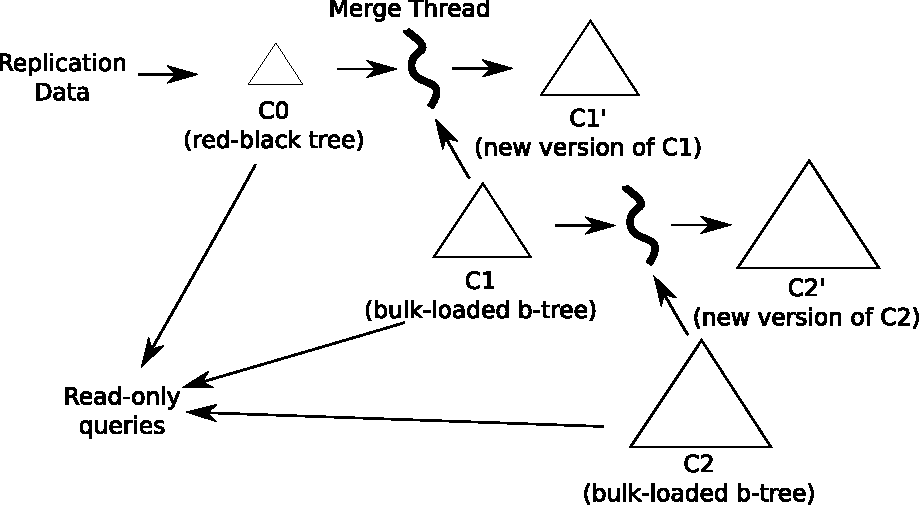
\epsfig{file=lsm-tree.pdf, width=3.33in}
\caption{The structure of a \rows LSM-tree}
\label{fig:lsm-tree}
\end{figure}
An LSM-Tree is an index that consists of multiple sub-trees called
{\em components} (Figure~\ref{fig:lsm-tree}).  The smallest component, $C0$, is a memory resident
binary search tree that is updated in place.  The next-smallest component, $C1$, is a bulk-loaded B-Tree.  As $C0$ grows,
it is merged with $C1$.  The merge process consists of index scans
and produces a new bulk-loaded version of $C1$ that contains the
updates from $C0$.  LSM-Trees can have arbitrarily many components,
though three (two on-disk tress) is generally adequate.
All other
components are produced by repeated merges with the next smaller
component.  Therefore, LSM-Trees are updated without resorting to
random disk I/O.

Lookups are performed by examining tree components, starting with the
in-memory (and most up-to-date) component, and then moving on
to progressively larger and out-of-date trees until a match is found.
This involves a maximum of two on-disk tree lookups unless a merge is
process, in which case three lookups may be required.

Unlike existing LSM-trees, \rows uses compression to increase merge
throughput.  Compression reduces the amount of sequential bandwidth
required by merges, trading surplus
computational power for scarce storage bandwidth.  Lookup performance
is determined by page cache hit ratios and the number of seeks
provided by the storage system.  \rowss compression increases the
effective size of the page cache.

\rowss second contribution is the application of LSM-trees to database
replication workloads.  In order to take full advantage of LSM-trees'
write throughput, the replication environment must not force \rows to
obtain pre-images of overwritten values.  Therefore, we assume that the
replication log records each transaction {\tt begin}, {\tt commit},
and {\tt abort} performed by the master database, along with the pre-
and post-images associated with each update.  The ordering of
these entries must match the order in which they are applied at the
database master.  Workloads that do not contain transactions or do not
update existing data may omit some of the mechanisms described here.

\rows focuses on providing inexpensive read-only queries to clients.
Instead of making each replicated transaction durable, \rows assumes
the replication log is made durable by some other mechanism.  \rowss
recovery routines ensure that some prefix of the replication log is
applied after a crash.  Replaying the remaining portion of the
replication log brings \rows up to date.  

\rows determines where to begin replaying the log by consulting its 
metadata.  Each time a new version of $C1$ is
completed, \rowss metadata is updated with the timestamp of the last
update to be applied to that version of $C1$.  This timestamp is that
of the last tuple written to $C0$ before the merge began.


Upon receiving a
log entry, \rows applies it to $C0$, and the update is immediately
available to queries that do not require a consistent view of the
data.  \rows provides snapshot consistency for readers that require
transactional isolation, making transactionally consistent data
available after a delay on the order of the duration of a few update
transactions.  All \rows transactions are read only and can
never block or abort due to reads or updates performed by other transactions.
Instead, long running read-only transactions delay the
deallocation of stale data, and long running updates introduce
replication delay.  Neither block \rowss maintenance tasks or index
operations.  The details of \rowss concurrency control mechanisms are
provided in Section~\ref{sec:isolation}.

%To prevent the in-memory tree from growing without bound, a merge
%process iterates over the (sorted) tree entries, and merges them with
%existing on-disk tree entries.  As the database increases in size, the
%on disk tree grows, forcing \rows to compare an ever-increasing number
%of existing tuples with each new tuple.  To mitigate this effect, the
%on-disk tree is periodically emptied by merging it with a second,
%larger tree.

\rows merges tree components in background threads, allowing
it to continuously process updates and service index lookup requests.
In order to minimize the overhead of thread synchronization, index
lookups latch entire tree components at a time.  Because on-disk tree
components are read-only, these latches only block reclamation of
space used by deallocated tree components.  $C0$ is
updated in place, preventing inserts from occurring concurrently with
lookups.  However, operations on $C0$ are comparatively
fast, reducing contention for $C0$'s latch.

Recovery, allocation and atomic updates to \rowss metadata are
handled by Stasis~\cite{stasis}, an extensible transactional storage
system.  \rows is implemented as a set of custom Stasis page formats
and tree structures.  Rather than commit each replicated transaction
independently, \rows creates one Stasis transaction per tree component
allocation and merge.  These transactions generate minimal log
information.

Redo and undo information for tree component metadata and headers are
written to the Stasis log, and tree component contents are force
written to the page file during Stasis commit.  During recovery,
partially written tree components are deallocated, and tree headers
are brought to a consistent state.  Tree component contents are never
written to log and are not manipulated during recovery.

After Stasis recovery completes, \rows is in a consistent state that
existed at some point in the past.  The replication log must be
played forward from that point in time in order to complete recovery.

%an extension to the transaction system and stores its
%data in a conventional database page file.  \rows does not use the
%underlying transaction system to log changes to its tree components.
%Instead, it force writes tree components to disk after each merge completes, ensuring
%durability without significant logging overhead.

%Stasis force writes \rows tree components to disk at commit, providing
%coarse-grained durability without generating a significant amount of
%log data.  Portions of \rows (such as tree component
%positions and index metadata) are updated in place and are stored using preexisting Stasis transactional
%storage primitives.  Tree components are allocated, written, and
%registered with \rows within a single Stasis transaction.  During
%recovery, any partially written \rows tree components are be
%deallocated and unregistered, leaving \rows in a consistent state.

%Stasis transactions are not visible to end users, and may contain many
%\rows transactions.  Therefore, after Stasis recovery completes, \rows
%uses the replication log to reapply any transactions lost because of the
%crash.

\subsection{Tree merging}

The remainder of this section provides an overview of LSM-Trees and quantifies the
cost of tuple insertions.  It then steps through a rough analysis of
LSM-Tree performance on current hardware.  Thorough analytical discussions of LSM
performance~\cite{lsm}, and comparisons between LSM-trees and a wide variety of other indexing techniques~\cite{partexp} are available elsewhere.  Next,
we explain how our implementation provides transactional isolation and
exploits hardware parallelism.  The adaptation of LSM-Trees to
database replication is an important contribution of this work and is
the focus of the rest of this section.  We defer discussion of
compression to the next section.

% XXX figures?
%An LSM-Tree consists of a number of underlying trees.
\rowss LSM-trees consist of three components.  Component zero ($C0$)
is an uncompressed in-memory binary search tree.  Components one and two ($C1$,
$C2$) are bulk-loaded compressed B-Trees.
%Only $C0$ is updated in place.
Each update is handled in three stages.  In the first stage,
it is applied to the in-memory tree.  Once enough updates
have been applied, a tree merge is initiated, and the tuple is
eventually merged with existing tuples in $C1$.  The merge process
performs a sequential scan over the in-memory tree and $C1$, producing
a new version of $C1$.

When the merge is complete, $C1$ is atomically replaced
with the new tree, and $C0$ is atomically replaced with an empty tree.
The process is eventually repeated when $C1$ and $C2$ are merged.

Replacing entire trees at once
introduces a number of performance problems.  In particular, it
doubles the number of bytes used to store each component, which is
important for $C0$, as it doubles memory requirements, and is
important for $C2$, as it doubles the amount of disk space used by
\rows.  Also, it forces index probes to access both versions of $C1$,
increasing random lookup times.

The original LSM work proposes a more sophisticated scheme that
addresses these issues by replacing one sub-tree at a time.  This
reduces peak storage and memory requirements but adds some complexity
by requiring in-place updates of tree components.

%Truly atomic replacement of portions of an LSM-Tree would cause ongoing
%merges to block insertions and force the mergers to run in lock step.
%We address this issue by allowing data to be inserted into
%the new version of the smaller component before the merge completes.
%This forces \rows to check both versions of components $C0$ and $C1$
%in order to look up each tuple, but it handles concurrency between merge steps
%without resorting to fine-grained latches. 

A third approach would partition \rows into multiple LSM-trees and
merge a single partition at a time.  This would reduce the frequency
of extra lookups caused by ongoing tree merges.  A similar approach is
evaluated in \cite{partexp}.

Partitioning also improves write throughput when updates are skewed,
as unchanged portions of the tree do not participate in merges and
frequently changing partitions can be merged more often.  We do not
consider these optimizations in the discussion below; including them
would complicate the analysis without providing any new insight.

\subsection{Amortized insertion cost}

In order to compute the amortized cost of insertion into an LSM-Tree,
we need only consider the cost of comparing the inserted tuple with
older tuples.  Otherwise, we would count the cost of each comparison
twice.  Therefore, we say that each tuple insertion ultimately causes
two rounds of I/O operations; one for the merge into $C1$, and another
to merge into $C2$.  Once a tuple reaches $C2$ it does not contribute
to the initiation of more I/O.  For simplicity, we assume the LSM-Tree
has reached a steady state.

%In a populated LSM-Tree $C2$ is the largest component, and $C0$ is the
%smallest component.  
The original LSM-Tree work proves that throughput
is maximized when the ratio of the sizes of $C1$ to $C0$ is equal to
the ratio between $C2$ and $C1$.  They call this ratio $R$.  Note that
for every $C0$ tuple consumed by a
merge, an average of $R$ tuples from $C1$ must be examined.  Similarly, each time a
tuple in $C1$ is consumed, $R$ tuples from $C2$ are examined.
Therefore, in a steady state:
\[size~of~tree\approx~R^2*|C0|\]
and:
\[insertion~rate*R(t_{C2}+t_{C1})\approx~sequential~i/o~cost\]
Where $t_{C1}$ and $t_{C2}$ are the amount of time it takes to read
from and write to C1 and C2.

%, insertion rate times the sum of $R *
%cost_{read~and~write~C2}$ and $R * cost_{read~and~write~C1}$ cannot
%exceed the drive's sequential I/O bandwidth.  Note that the total size
%of the tree is approximately $R^2 * |C0|$.
% (neglecting the data stored
%in $C0$ and $C1$)\footnote{The proof that keeping R constant across
%  our three tree components follows from the fact that the mergers
%  compete for I/O bandwidth and $x(1-x)$ is maximized when $x=0.5$.
%  The LSM-Tree paper proves the general case.}.

\subsection{Replication Throughput}

LSM-Trees have different asymptotic performance characteristics than
conventional index structures.  In particular, the amortized cost of
insertion is $O(\sqrt{n})$ in the size of the data and is proportional
 to the cost of sequential I/O.  In a B-Tree, this cost is
$O(log~n)$ but is proportional to the cost of random I/O.
%The relative costs of sequential and random
%I/O determine whether or not \rows is able to outperform B-Trees in
%practice.
This section describes the impact of compression on B-Tree
and LSM-Tree performance using simplified models of
their performance characteristics.

In particular, we assume that the leaf nodes do not fit in memory, and
that tuples are accessed randomly with equal probability.  To simplify
our calculations, we assume that internal tree nodes fit in RAM.
Without a skewed update distribution, reordering and batching I/O into
sequential writes only helps if a significant fraction of the tree's
data fits in RAM.  Therefore, we do not consider B-Tree I/O batching here.

%If we assume uniform access patterns, 4 KB pages and 100 byte tuples,
%this means that an uncompressed B-Tree would keep $\sim2.5\%$ of the
%tuples in memory.  Prefix compression and a skewed update distribution
%would improve the situation significantly, but are not considered
%here.
Starting with the more familiar B-Tree case, in the steady state we
can expect each index update to perform two random disk accesses: one
evicts a page; the other reads a page.  Tuple compression does not
reduce the number of disk seeks:
\[
   cost_{Btree~update}=2~cost_{random~io}
\]
In \rows, we have:
\[
   cost_{LSMtree~update}=2*2*2*R*\frac{cost_{sequential~io}}{compression~ratio}  %% not S + sqrt S; just 2 sqrt S.
\]
We multiply by $2R$ because each new
tuple is eventually merged into both on-disk components, and
each merge involves $R$ comparisons with existing tuples on average.

The second factor of two reflects the fact that the merger must read
existing tuples into memory before writing them back to disk.
An update of a tuple is handled as an insertion of the new
tuple and a deletion of the old tuple.  Deletion is simply an insertion
of a tombstone tuple, leading to the third factor of two.

Updates that do not modify primary key fields avoid this final factor
of two.  If update is an atomic operation then the delete and insert
will always occur during the same snapshot.  Since the delete and
insert share the same primary key and the same snapshot number, the
insertion will always supercede the deletion.  Therefore, there is no
need to insert a tombstone.

%
% Merge 1:
%  read C1 R times, write C1 R times.
%
% Merge 2:
%  read C1 1 times
%  read C2 R times, write C2 R times.
%

The $compression~ratio$ is
$\frac{uncompressed~size}{compressed~size}$, so improved compression
leads to less expensive LSM-Tree updates.  For simplicity, we assume
that the compression ratio is the same throughout each component of
the LSM-Tree; \rows addresses this at run-time by reasoning in terms
of the number of pages used by each component.

Our test hardware's hard drive is a 7200RPM, 750 GB Seagate Barracuda
ES.  
%has a manufacturer-reported average rotational latency of
%$4.16~msec$, seek times of $8.5/9.5~msec$ (read/write), and a maximum
%sustained throughput of $78~MB/s$.  
Third party
benchmarks\cite{hdBench} %\footnote{http://www.storagereview.com/ST3750640NS.sr}
report random access times of 12.3/13.5~msec (read/write) and 44.3-78.5~megabytes/sec
sustained throughput.  Timing {\tt dd if=/dev/zero of=file; sync} on an
empty ext3 file system suggests our test hardware provides 57.5~megabytes/sec of
storage bandwidth, but running a similar test via Stasis' buffer manager produces
inconsistent results ranging from 22 to 47~megabytes/sec.

%We used two hard drives for our tests, a smaller, high performance drive with an average seek time of $9.3~ms$, a
%rotational latency of $4.2~ms$, and a manufacturer reported raw
%throughput of $150~mb/s$.  Our buffer manager achieves $\sim 27~mb/s$
%throughput; {\tt dd if=/dev/zero of=file} writes at $\sim 30.5~mb/s$.

Assuming a fixed hardware configuration, and measuring cost in disk
time, we have:
%\[
%   cost_{sequential~io}=\frac{|tuple|}{30.5*1024^2}=0.000031268~msec
%\]
%% 12.738854
\[
   cost_{sequential}=\frac{|tuple|}{78.5MB/s}=12.7~|tuple|~~nsec/tuple~(min)
\]
%% 22.573363
\[
   cost_{sequential}=\frac{|tuple|}{44.3MB/s}=22.6~|tuple|~~nsec/tuple~(max)
\]
and
\[
   cost_{random}=\frac{12.3+13.5}{2} = 12.9~msec/tuple
\]
Pessimistically setting
\[
2~cost_{random}\approx1,000,000\frac{cost_{sequential}}{|tuple|}
\] yields: \[
    \frac{cost_{LSMtree~update}}{cost_{Btree~update}}=\frac{2*2*2*R*cost_{sequential}}{compression~ratio*2*cost_{random}}
%   \frac{cost_{LSMtree~update}}{cost_{Btree~update}} \approx \frac{(S + \sqrt{S})}{|tuple|~compression~ratio~250,000}
\]
\[
   \approx\frac{R*|tuple|}{250,000*compression~ratio}
\]
If tuples are 100 bytes and we assume a compression ratio of 4, which is lower
than we expect to see in practice, but numerically convenient, then the
LSM-Tree outperforms the B-Tree when:
\[
    R < \frac{250,000*compression~ratio}{|tuple|}
\]
\[
    R < 10,000
\]
%750 gb throughput = 1 / (((8 * 27 * 22.6 * 100) / 4) * (ns)) = 8.00198705 khz
% 1 / (((8 * 2.73 * 100 * 22.6) / 4) * (ns))
on a machine that can store 1 GB in an in-memory tree.
%, this yields a
%maximum ``interesting'' tree size of $R^2*1GB = $ 100 petabytes, well
%above the actual drive capacity of $750~GB$.
  A 750~GB tree would
have a $C2$ component 750 times larger than the 1GB $C0$ component.
Therefore, it would have an $R$ of $\sqrt{750}\approx27$; we would
expect such a tree to have a sustained insertion throughput of
approximately 8000~tuples/sec, or 800~kilobytes/sec
%\footnote{It would
%  take 11 days to overwrite every tuple on the drive in random order.}
given our 100 byte tuples.

Our hard drive's average access time allows the drive to deliver 83 I/O operations/sec.
Therefore, we can expect an insertion throughput of 41.5~tuples/sec from a B-Tree with
a 18.5~GB buffer pool.  With just 1~GB of RAM, \rows should outperform the
B-Tree by more than two orders of magnitude.  Increasing \rowss system
memory to cache 10~GB of tuples would increase write performance by a
factor of $\sqrt{10}$.

% 41.5/(1-80/750) = 46.4552239

Increasing memory another ten fold to 100~GB would yield an LSM-Tree
with an R of $\sqrt{750/100} = 2.73$ and a throughput of 81,000~tuples/sec.
In contrast, the B-Tree would cache less than 100~GB of leaf pages
in memory and would write fewer than $\frac{41.5}{1-(100/750)} = 47.9$
tuples/sec.  Increasing memory further yields a system that
is no longer disk bound.

Assuming CPUs are fast enough to allow \rowss
compression and merge routines to make use of the bandwidth supplied
by the disks, we conclude that \rows will provide significantly higher
throughput than a seek-bound B-Tree.

\subsection{Indexing}

Our analysis ignores the cost of allocating and initializing
LSM-Trees' internal nodes.  The merge process uses compressed pages as
tree leaf pages.  Each time the compression process fills a page it
inserts an entry into the leftmost entry in the tree, allocating
additional internal nodes if necessary.  Our prototype does not
compress internal tree nodes.

The space overhead of building these tree nodes depends on the number
of tuples that fit in each page.  If tuples are small, \rows gets good
fan-out on internal nodes, reducing the fraction of storage reserved
for tree pages.  \rows inherits a default page size of 4KB from
Stasis.  Although this is fairly small by modern standards, even with
4KB pages, \rowss per-page overheads are acceptable.  For the tuple
sizes used in our experiments tree node overhead amounts to a few
percent.  For larger, or very compressible tuples, tree overhead can
be more significant.

Consider a tree that can store 10 compressed tuples in each 4K page.
If an uncompressed tuple is 400 bytes long, then roughly a tenth of
the pages are dedicated to the lowest level of tree nodes, with a
tenth that number devoted to the next highest level, and so on.  With
a 2x compression ratio, uncompressed tuples occupy 800 bytes and each
higher level in the tree is only a fifth the size of the level below
it.  Larger page sizes and compression of internal nodes would reduce
the overhead of tree creation.

%Table~\ref{table:treeCreationTwo} provides a comparison of compression
%performance with and without tree creation enabled\footnote{Our
%  analysis ignores page headers, per-column, and per-tuple overheads;
%  these factors account for the additional indexing overhead.}.  The
%data was generated by applying \rowss compressors to randomly
%generated five column, 1,000,000 row tables.  Across five runs, in
%Table~\ref{table:treeCreation} RLE's page count had a standard
%deviation of $\sigma=2.35$; the other page counts had $\sigma=0$.  In
%Table~\ref{table:treeCreationTwo}, $\sigma < 7.26$ pages.

%Throughput's $\sigma<6MB/s$.


%% As the size of the tuples increases, the number of compressed pages
%% that each internal tree node points to decreases, increasing the
%% overhead of tree creation.  In such circumstances, internal tree node
%% compression and larger pages should improve the situation.

\subsection{Isolation}
\label{sec:isolation}

\rows must deal with two types of transactions: updates from the
master and the read-only queries it provides to its clients.  \rows
has no control over the order or isolation of updates from the master
database, so it must apply these updates in an order consistent with
the master database order.  LSM-tree updates do not immediately remove
pre-existing data from the tree.  Instead, they provide a simple form
of versioning, where data from the newest component ($C0$) is always
the most up to date.  We extend this idea to provide snapshots.  Each
transaction is assigned to a snapshot, and no more than one version of
each tuple exists within a snapshot.

To lookup a tuple as it existed at some point in time, we examine all
snapshots that were taken before that point and return the most recent
version of the tuple that we find.  All versions of the same tuple are
stored in adjacent positions in the LSM-tree, so this is an
inexpensive operation.  Furthermore, \rowss versioning is meant to be
used for transactional consistency, and not time-travel.  This should
restrict the number of snapshots to a manageable level.

In order to insert a tuple \rows first determines which snapshot the
tuple should belong to.  At any given point in time up to two snapshots
may accept new updates.  The newer of these snapshots accepts new
transactions.  If the replication log contains interleaved transactions,
the older snapshots waits for any pending transactions that
it contains to complete.  Once all of those transactions are complete,
the older snapshot will stop accepting updates, the newer snapshot
will stop accepting new transactions, and a snapshot for new
transactions will be created.

\rows examines the time stamp and transaction id associated with the tuple insertion,
and marks the tuple with the appropriate snapshot number.  It then
inserts the tuple into $C0$, overwriting any tuple that matches on
primary key and has the same snapshot id.

When it is time to merge the inserted tuple with $C1$, the merge
thread consults a list of currently accessible snapshots.  It uses this
to decide which versions of the tuple in $C0$ and $C1$ are accessible
to transactions.  Such versions are the most recent versions that
existed before the end of an accessible snapshot.  After finding all
such versions of a tuple (one may exist for each accessible snapshot),
the merge process writes them to the new version of $C1$.  Any other
versions of the tuple are discarded.  If two matching tuples from the
same snapshot are encountered, one must be from $C0$ and the other
from $C1$.  The merger discards the version from $C1$, since $C0$ is
more recent.  An identical procedure is followed when insertions from
$C1$ and $C2$ are merged.

\rows handles tuple deletion by inserting a tombstone.  Tombstones
record the deletion event and are handled similarly to insertions.  A
tombstone will be kept if is the newest version of a tuple in at least one
accessible snapshot.  Otherwise, the tuple can be deleted because it
 was reinserted after the deletion but before the next accessible
snapshot was taken.  Unlike insertions, tombstones in
$C2$ can be deleted if they are the oldest remaining reference to a tuple.

%% The correctness of \rows snapshots relies on the isolation mechanisms
%% provided by the master database.  Within each snapshot, \rows applies
%% all updates in the same order as the primary database and cannot lose
%% sync with the master.  However, across snapshots, concurrent
%% transactions can write non-conflicting tuples in arbitrary orders,
%% causing reordering of updates.  These updates are guaranteed to be
%% applied in transaction order.  If the master misbehaves and applies
%% conflicting updates out of transaction order then \rows and the
%% master's version of the database will lose synchronization.  Such out
%% of order updates should be listed as separate transactions in the
%% replication log.

%% If the master database provides snapshot isolation using multiversion
%% concurrency control, \rows can reuse the timestamp the database
%% applies to each transaction.  If the master uses two phase locking,
%% the situation becomes more complex, as \rows has to use the commit time
%% (the point in time when the locks are released) of each transaction.

%% Until the commit time is known, \rows would store the transaction id
%% in the LSM-Tree.  As transactions are committed it would record the
%% mapping from transaction id to snapshot.  Eventually, the merger would
%% translate transaction ids to snapshots, preventing the mapping from
%% growing without bound.

\rowss snapshots have minimal performance impact and provide
transactional concurrency control without blocking or rolling back
transactions.  Also, they do not block \rowss merge and replication
processes.  However, long running updates prevent queries from
accessing the results of recently completed transactions, causing the
results that \rows returns to become increasingly stale.  Long running
queries increase the number of accessible snapshots, increasing \rowss
disk footprint.  Both issues can be partially addressed by limiting
the length of transactions.

%\label{sec:isolation}
%\rows combines replicated transactions into snapshots.  Each transaction
%is assigned to a snapshot according to a timestamp; two snapshots are
%active at any given time.  \rows assigns incoming transactions to the
%newer of the two active snapshots.  Once all transactions in the older
%snapshot have completed, that snapshot is marked inactive, exposing
%its contents to new queries that request a consistent view of the
%data.  At this point a new active snapshot is created, and the process
%continues.

%(XXX explain life of tuple here)

%%The timestamp is simply the snapshot number.
%In the case of a tie
%during merging, such as two tuples with the same primary key and
%timestamp, the version from the newer (lower numbered) component is
%taken.  If a tuple maintains the same primary key while being updated
%multiple times within a snapshot, this allows \rows to discard all but
%the last update before writing the tuple to disk.

%New snapshots are created in two steps.  First, all transactions in
%epoch $t-1$ must complete (commit or abort) so that they are
%guaranteed to never apply updates to the database again.  In the
%second step, \rowss current snapshot number is incremented, new
%read-only queries are assigned to snapshot $t-1$, and new updates
%are assigned to snapshot $t+1$.  Each such query is granted a
%shared lock on the existence of the snapshot, protecting that version
%of the database from garbage collection.  In order to ensure that new
%snapshots are created in a timely and predictable fashion, the time
%between them should be acceptably short, but still slightly longer
%than the longest running transaction.  Using longer snapshots
%increases coalescing of repeated updates to the same tuples,
%but increases replication delay.
%
%\subsubsection{Isolation performance impact}
%
%Although \rowss isolation mechanisms never block the execution of
%index operations or merge processes, their behavior degrades in the presence of long
%running transactions.
%
%Long running updates do not prevent tree merges from continuing,
%but they can block the creation of new snapshots.  Upon
%encountering such a transaction, \rows can either wait or ask the
%master database to abort the offending transaction, then wait until
%appropriate rollback (or commit) entries appear in the replication
%log.  While waiting for a long running transaction in snapshot $t-1$
%to complete, \rows continues to process replication requests by
%extending snapshot $t$, and services requests for consistent data from
%the increasingly stale snapshot $t-2$.
%
%%simply asks the master database to abort the offending update.  It
%%then waits until appropriate rollback (or perhaps commit) entries
%%appear in the replication log, and creates the new snapshot.  While
%%waiting for the transactions to complete, \rows continues to process
%%replication requests by extending snapshot $t$.
%
%%Of course, proactively aborting long running updates is simply an
%%optimization.  Without a surly database administrator to defend it
%%against application developers, \rows does not send abort requests,
%%but otherwise behaves identically.  Read-only queries that are
%%interested in transactional consistency continue to read from (the
%%increasingly stale) snapshot $t-2$ until $t-1$'s long running
%%updates commit.
%
%Long running queries present a different set of challenges to \rows.
%%Although \rows provides fairly efficient time-travel support,
%%versioning databases are not our target application.  \rows
%%provides each new read-only query with guaranteed access to a
%%consistent version of the database.
%They force \rows to keep old versions of overwritten tuples around
%until the query completes.  These tuples increase the size of \rowss
%LSM-Trees, increasing merge overhead.  If the space consumed by old
%versions of the data is a serious issue, extremely long running
%queries should be disallowed.  Alternatively, historical or
%long-running queries could be run against certain snapshots (every
%1000th, or the first one of the day, for example), reducing the
%number of snapshots maintained by \rows.
%
%\subsubsection{Merging and Garbage collection}
%
%\rows merges components by iterating over them in order, garbage collecting
%obsolete and duplicate tuples and writing the rest into a new version
%of the larger component.  Because \rows provides snapshot consistency
%to queries, it must be careful not to collect a version of a tuple that
%is visible to any outstanding or future query.  \rows
%deletes data by
%inserting special tombstone tuples into the tree.  A tombstone's
%purpose is to record the deletion event until all older versions of
%the tuple have been garbage collected.  Sometime after that point, the tombstone
%is collected as well.
%
%(XXX clarify this paragraph) In order to determine whether or not a tuple can be collected, \rows
%compares the tuple's timestamp with any matching tombstones, and with any tuples that
%match on primary key.  Upon encountering such candidates for garbage collection,
%\rows compares their timestamps with the set of locked snapshots.  If
%there are no snapshots between the tuple being examined and the
%updated version, then the tuple can be collected.  Tombstone tuples can
%also be collected once they reach $C2$ and any older matching tuples
%have been removed.
%
%Actual reclamation of pages is handled by Stasis; each time a tree
%component is replaced, \rows simply tells Stasis to free the regions of
%pages that contain the obsolete tree.
%
%%the underlying transaction
%%system; once \rows completes its scan over existing components (and
%%registers new ones in their places), it tells the transaction system
%%to reclaim the regions of the page file that stored the old components.

\subsection{Parallelism}

All \rows operations are concurrent; readers and writers work
independently, avoiding blocking, deadlock and livelock.  Index probes
must latch $C0$ in order to perform a lookup, but the more costly
probes into $C1$ and $C2$ are against read-only trees.  Beyond locating
and pinning tree components against deallocation, probes of these
components do not interact with the merge processes.

Each component's merge process runs in a separate thread.  This
allows our prototype to exploit two to three processor cores while
inserting and recompressing data during replication.  Remaining cores
could be exploited by range partitioning a replica into multiple
LSM-trees, allowing more merge processes to run concurrently.
Therefore, we expect the throughput of \rows replication to increase
with memory size, compression ratios and I/O bandwidth for the foreseeable future.

%[XXX need experimental evidence...]  During bulk
%load, the buffer manager, which uses Linux's {\tt sync\_file\_range}
%function allows \rows to asynchronously force regions [XXX currently,
%  we do a synchronous force with sync\_file\_range....] of the page
%file to disk.  \rows has control over region size; if the system is
%CPU bound \rows can ensure that the time spent waiting for synchronous
%page writes is negligible, by choosing an appropriate region size.  On
%the other hand, if the system is disk bound, the same asynchronous
%force mechanism ensures that \rows overlaps computation with I/O. [XXX
% this is probably too detailed; we should just say that \rows uses
% standard techniques to overlap computation and I/O]

%% \subsection{Recovery}

%% Like other log structured storage systems, \rowss recovery process is
%% inexpensive and straightforward.  However, \rows does not attempt to
%% ensure that transactions are atomically committed to disk, and is not
%% meant to replace the master database's recovery log.

%% Instead, recovery occurs in two steps.  Whenever \rows writes a tree
%% component to disk, it does so by beginning a new transaction in the
%% underlying transaction system.  Next, it allocates
%% contiguous regions of disk pages (generating one log entry per
%% region), and performs a bulk load of the new tree into
%% these regions (this bulk load does not produce any log entries).
%% Then, \rows forces the tree's regions to disk, and writes the list
%% of regions used by the tree and the location of the tree's root to
%% normal (write ahead logged) records.  Finally, it commits the
%% underlying transaction.

%% After the underlying transaction system completes recovery, \rows
%% will have a set of intact and complete tree components.  Space taken
%% up by partially written trees was allocated by an aborted
%% transaction, and has been reclaimed by the transaction system's
%% recovery mechanism.  After the underlying recovery mechanisms
%% complete, \rows reads the last committed timestamp from the LSM-Tree
%% header, and begins playback of the replication log at the appropriate
%% position.  Upon committing new components to disk, \rows allows the
%% appropriate portion of the replication log to be truncated.

\section{Row compression}

\begin{table}
\caption{Compression ratios and index overhead - five columns (20 bytes/column)}
\centering
\label{table:treeCreation}
\begin{tabular}{|l|c|c|c|} \hline
Format     & Compression & Page count \\ \hline %& Throughput\\ \hline
PFOR        & 1.96x       & 2494       \\ \hline %& 133.4 MB/s \\ \hline
PFOR + tree & 1.94x       & +80        \\ \hline %& 129.8 MB/s \\ \hline
RLE        & 3.24x       & 1505 \\ \hline %& 150.6 MB/s \\ \hline
RLE + tree & 3.22x       & +21        \\  %& 148.4 MB/s \\
\hline\end{tabular}
\end{table}
\begin{table}
\caption{Compression ratios and index overhead - 100 columns (400 bytes/column)}
\centering
\label{table:treeCreationTwo}
\begin{tabular}{|l|c|c|c|} \hline
Format     & Compression & Page count \\ \hline %& Throughput\\ \hline
PFOR        & 1.37x       & 7143       \\ \hline %& 133.4 MB/s \\ \hline
PFOR + tree & 1.17x       & 8335        \\ \hline %& 129.8 MB/s \\ \hline
RLE        & 1.75x       & 5591 \\ \hline %& 150.6 MB/s \\ \hline
RLE + tree & 1.50x       & 6525        \\  %& 148.4 MB/s \\

\hline\end{tabular}
\end{table}


\rows stores tuples in a sorted, append-only format.  This greatly
simplifies compression and provides a number of new opportunities for
optimization.  Compression reduces sequential I/O, which is \rowss primary bottleneck.
It also
increases the effective size of the buffer pool, allowing \rows to
service larger read sets without resorting to random I/O.

Row-oriented database compression techniques must cope with random,
in-place updates and provide efficient random access to compressed
tuples.  In contrast, compressed column-oriented database layouts
focus on high-throughput sequential access and do not provide in-place
updates or efficient random access.  \rows never updates data in
place, allowing us to make use of append-only compression techniques
from the column literature.  Also, \rowss tuples never span pages, and
are stored in sorted order.  We adapt column compression techniques to provide an
index over the page contents, providing efficient random access within
pages.

\rowss compression format is straightforward.  Each page is divided into
a header, a set of compressed segments and a single exception section
(Figure~\ref{fig:mc-fmt}).  There is one compressed segment per column
and each such segment may be managed by a different compression
algorithm, which we call a {\em compressor}.  Some compressors cannot
directly store all values that a column may take on.  Instead, they
store such values in the exception section.  We call
\rowss compressed page format the {\em multicolumn} format, and have
implemented it to support efficient compression,
decompression and random lookups by slot id and by value.

\subsection{Compression algorithms}
Our prototype provides three compressors.  The first, {\em NOP},
simply stores uncompressed integers.  The second, {\em RLE},
implements run length encoding, which stores values as a list of
distinct values and repetition counts.  The third, {\em PFOR}, or
patched frame of reference, stores values as a single per-page
base offset and an array of deltas~\cite{pfor}.  The values are reconstructed by
adding the offset and the delta or by traversing a pointer into the
exception section of the page.  Currently \rows only supports integer
data, but could be easily extended with support for strings and
other types.  Also, the compression algorithms that we
implemented would benefit from a technique known as {\em bit-packing},
which represents integers with lengths other than 8, 16, 32 and 64
bits.  Bit-packing would increase \rowss compression ratios,
and can be implemented with a modest performance overhead~\cite{pfor}.

%(XXX this paragraph makes no sense; it's been moved out of context...)
%We implemented two compression formats for \rowss multicolumn pages.
%The first is PFOR; the other is {\em run length encoding} (RLE), which
%stores values as a list of distinct values and repetition counts.
We chose these techniques because they are amenable to optimization;
our implementation makes heavy use of C++ templates, static code
generation and g++'s optimizer in order to keep \rows from becoming
CPU-bound.  By hardcoding table formats at compilation time, this
implementation removes length and type checks, and allows the compiler
to inline methods, remove temporary variables and optimize loops.

\rows includes a second, less efficient implementation that uses
dynamic method dispatch to support runtime creation of new table
schemas.  A production-quality system could use runtime code
generation to support creation of new schemas while taking full
advantage of the compiler's optimizer.

\subsection{Comparison with other approaches}

\rowss tuples never span multiple pages, and pages are partitioned by
column, as in the PAX page format.  Partitioning pages by column
improves processor cache locality for queries that do not need to
examine every column within a page.  In particular, many queries
filter based on the value of a few attributes.  If data is clustered
into rows, then each column from the page will be brought into cache,
even if no tuples match.  By clustering data into columns, PAX ensures
that only the necessary columns are brought into cache\cite{PAX}.

\rowss use of lightweight compression algorithms is similar to
approaches used in column databases\cite{pfor}.  \rows differs from
that work in its focus on efficient random reads on commodity
hardware.  Existing work targeted RAID and used page sizes ranging from 8-32MB.  Rather
than use large pages to get good sequential I/O performance, \rows
uses 4KB pages and relies upon automatic prefetch and write coalescing
provided by Stasis' buffer manager and the underlying operating
system.  This reduces the amount of data handled by \rows during index
probes.

\subsection{Tuple lookups}

Because we expect index lookups to be a frequent operation, our
page format supports efficient lookup by tuple value.  The original
``patched'' compression algorithms store exceptions in a linked list
and perform scans of up to 128 tuples in order to materialize compressed
tuples.  This was done in order to reduce the number of branches
required during compression and sequential decompression.  We
investigated a number of implementations of tuple lookup by value
including per-column range scans and binary search.  \xxx{need data here}

The efficiency of random access within a
page depends on the format used by column compressors.  \rows
compressors support two access methods.  The first looks up a value by
slot id.  This operation is $O(1)$ for frame of reference columns, and
$O(log~n)$ in the number of runs of identical values on the page for
run length encoded columns.

The second operation is used to look up tuples by value and is based
on the assumption that the the tuples are stored in the
page in sorted order.  The simplest way to provide access to tuples by
value would be to perform a binary search, materializing each tuple
that the search needs to examine.  Doing so would materialize many
extra column values, potentially performing additional binary searches.

To lookup a tuple by value, the second operation takes a range of slot
ids and a value, and returns the offset of the first and last instance
of the value within the range.  This operation is $O(log~n)$ in the
number of slots in the range for frame of reference columns, and
$O(log~n)$ in the number of runs on the page for run length encoded
columns.  The multicolumn implementation uses this method to look up
tuples by beginning with the entire page in range and calling each
compressor's implementation in order to narrow the search until the
correct tuple(s) are located or the range is empty.
Partially-matching tuples are only partially decompressed during the
search, reducing the amount of data brought into processor cache.

%(XXX future work:)
%
%Compressed \rows pages provide access to their data in three ways: via
%an iterator, by slot id, and by value.  Page iterators store
%information about the next tuple to be returned, minimizing branches
%and guaranteeing O(1) access to the next value.  \rowss page format is
%able to support the techniques of~\cite{XXX}, which provide vectors of
%tuples depending on the nature of the operator scanning over the page,
%but we chose not to implement this.
%
%To materialize a tuple based on its slot id (logical position on the
%page), we ask the compression algorithm responsible for each
%column to return the appropriate value.  For some compression
%algorithms this is a simple array lookup, while for others (such as
%run length encoding) the procedure involves a binary search.
%
%\rows is also able to lookup tuples by value.  Tuples are always
%stored in sorted order, first on the first column, then on the second
%and so on.  The simplest way to look up a tuple by value would be to
%perform a binary search, materializing each tuple that the search
%needs to examine.  Doing so would materialize many extra column
%values.  Since these column values are compressed, each tuple
%materialization could involve multiple binary searches.
%
%Instead, \rowss compression implementations provide search methods
%that take a column value and a range of slot ids.  To lookup a tuple,
%we first perform a search for the appropriate value on the entire
%first column.  This returns a range of candidate tuple ids.  Since each
%of these tuples has the same value in its first column, we know the
%second column is sorted within the range.  Therefore, we can
%efficiently search the second column of the candidate range.  We
%repeat this procedure until the range becomes empty (and no match is
%found), or until all columns have been matched.  This reduces the
%number of operations that must be performed while looking up a tuple,
%and also reduces the amount of data brought into CPU cache.

%% More stuff ->

%\rows uses compression to improve performance.  Conserving storage space is of
%%secondary concern.  Sequential I/O throughput is \rowss primary
%replication and table scan bottleneck, and is proportional to the
%compression ratio.  Compression increases the effective
%size of the buffer pool and therefore, the size of the largest read set
%\rows can service without resorting to random I/O.

%Because \rows never updates data in place, it
%is able to make use of read-only compression formats that cannot be
%efficiently applied to B-Trees.

%% Disk heads are the primary
%% storage bottleneck for most OLTP environments, and disk capacity is of
%% secondary concern.  Therefore, database compression is generally
%% performed to improve system performance, not capacity.  In \rows,
%% sequential I/O throughput is the primary replication bottleneck; and
%% is proportional to the compression ratio.

%This allows us to service small updates using
%techniques from column-oriented databases.  This is because, like column-oriented
%databases, \rows can provide sorted, projected data to bulk-loaded indexes.

%\rowss compression formats are based on our
%{\em multicolumn} compression format.  In order to store data from
%an $N$ column table, we divide the page into $N+1$ variable length
%regions.  $N$ of these regions each contain a compressed column.  The
%remaining region contains ``exceptional'' column data (Figure~\ref{fig:mc-fmt}).

\begin{figure}
\centering 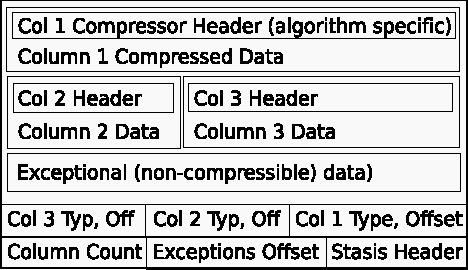
\epsfig{file=multicolumn-page-format.pdf, width=3in}
\caption{Multicolumn page format.  Many compression algorithms
can coexist on a single page.  Tuples never span multiple pages.}
\label{fig:mc-fmt}
\end{figure}

%For example, a column might be encoded using the {\em frame of
%  reference} (FOR) algorithm, which stores a column of integers as a
%single offset value and a list of deltas.  When a value too different
%from the offset to be encoded as a delta is encountered, an offset
%into the exceptions region is stored.  When applied to a page that
%stores data from a single column, the resulting algorithm is MonetDB's
%{\em patched frame of reference} (PFOR)~\cite{pfor}.

%\rowss multicolumn pages extend this idea by allowing multiple columns
%(each with its own compression algorithm) to coexist on each page and preventing tuples from spanning pages.
%This reduces the cost of reconstructing tuples during index lookups.

%This section discusses the computational and storage overhead of our
%multicolumn compression approach.  We suspect this technique has been
%used in the past.  However, this type of compression format is
%conspicuously absent in the recent literature, and represents a
%different set of tradeoffs than other current approaches.

\subsection{Multicolumn computational overhead}

%sears@davros:~/stasis/benchmarks$ ./rose -n 10 -p 0.01
%Compression scheme: Time trial (multiple engines)
%Page size:          4096
%P(bump):            0.010000
%Random seed:        0
%Column count:       10

%WARNING: Pstar will only use the first column.

%Compression scheme   #pages      ratio  comp gb/s  decom gb/s
%Pstar        (For)      493      3.96x      0.544       2.982
%Multicolumn  (For)     5129      3.81x      0.253       0.712
%Pstar        (Rle)       40     48.83x      0.961       1.593
%Multicolumn  (Rle)      416     46.95x      0.377       0.692

\begin{table}
\caption{Compressor throughput - Random data Mean of 5 runs, $\sigma<5\%$, except where noted}
\centering
\label{table:perf}
\begin{tabular}{|l|c|c|c|} \hline
Format        & Ratio & Compress  & Decompress\\ \hline %& Throughput\\ \hline
PFOR - 1 column    &    3.96x  &  547 mb/s &    2959 mb/s \\ \hline %& 133.4 MB/s \\ \hline
PFOR - 10 column   &    3.86x  &  256 &      719 \\ \hline %& 129.8 MB/s \\ \hline
RLE - 1 column     &   48.83x  &  960  &    1493 $(12\%)$ \\ \hline %& 150.6 MB/s \\ \hline
RLE - 10 column    &   47.60x  &  358 $(9\%)$ & 659 $(7\%)$ \\  %& 148.4 MB/s \\
\hline\end{tabular}
\end{table}


Our multicolumn page format introduces additional computational
overhead in two ways.  First, \rows compresses each column in a
separate buffer, then uses {\tt memcpy()} to gather this data into a
single page buffer before writing it to disk.  This {\tt memcpy()}
occurs once per page allocation.

Bit-packing is typically implemented as a post-processing
technique that makes a pass over the compressed data~\cite{pfor}.  \rowss
gathering step can be performed for free by such a bit-packing
implementation, so we do not see this as a significant disadvantage
compared to other approaches.

Second, we need a way to translate tuple insertions into
calls to appropriate page formats and compression implementations.
Unless we hardcode the \rows executable to support a predefined set of
page formats and table schemas, each tuple compression and decompression operation must execute an extra {\tt for} loop
over the columns.  The for loop's body contains a {\tt switch} statement that chooses between column compressors, since each column can use a different compression algorithm and store a different data type.

This form of multicolumn support introduces significant overhead;
these variants of our compression algorithms run significantly slower
than versions hard-coded to work with single column data.
Table~\ref{table:perf} compares a fixed-format single column page
layout with \rowss dynamically dispatched (not custom generated code)
multicolumn format. \xxx{any way to compare with static page layouts??}

% explain how append works

\subsection{The {\tt \large append()} operation}

\rowss compressed pages provide a {\tt tupleAppend()} operation that
takes a tuple as input and returns {\tt false} if the page does not have
room for the new tuple.  {\tt tupleAppend()} consists of a dispatch
routine that calls {\tt append()} on each column in turn.
%Each
%column's {\tt append()} routine secures storage space for the column
%value, or returns {\tt false} if no space is available.
{\tt append()} has the
following signature:
%\begin{quote}
\begin{verbatim}
void append(COL_TYPE value, int* exception_offset,
    void* exceptions_base, void* column_base,
    int* freespace)
\end{verbatim}
%\end{quote}
where {\tt value} is the value to be appended to the column, {\tt
  exception\_offset} is a pointer to the offset of the first free byte in the
exceptions region, and {\tt exceptions\_base} and {\tt column\_base} point
to page-sized buffers used to store exceptions and column data as
the page is being written.  One copy of these buffers exists for
each page that \rows is actively writing to (one per disk-resident
LSM-Tree component); they do not significantly increase \rowss memory
requirements.

{\tt freespace} is a pointer to the number of free bytes
remaining on the page.  The multicolumn format initializes these
values when the page is allocated.  As {\tt append()} implementations
are called they update this data accordingly.  Each time a column
value is written to a page the column compressor must allocate some
space to store the new value.  A naive allocation approach would have
the compressor check {\tt freespace} to decide if the page is full,
and return an error code otherwise.  Then its caller would check the
return value, and behave appropriately.  This would lead to two branches
per column value, greatly decreasing compression throughput.

We avoid these branches by reserving a portion of the page (typically the
size of a single incompressible tuple) for speculative allocation.
Instead of checking for freespace, compressors decrement the current
freespace count and append data to the end of their segment.
Once an entire tuple has been written to a page,
it checks the value of freespace and decides if another tuple may be
safely written.  This also simplifies corner cases; if a
compressor cannot store more tuples on a page, but has not run out of
space\footnote{This can happen when a run length encoded page stores a
  very long run of identical tuples.} it simply sets {\tt
  freespace} to -1 then returns.

%% Initially, our multicolumn module managed these values
%% and the exception space.  This led to extra arithmetic operations and
%% conditionals and did not significantly simplify the code.  Note that,
%% compared to techniques that store each tuple contiguously on the page,
%% our format avoids encoding the (variable) length of each tuple; instead
%% it encodes the length of each column.

% contrast with prior work

The original PFOR implementation~\cite{pfor} assumes it has access to
a buffer of uncompressed data and that it is able to make multiple
passes over the data during compression.  This allows it to remove
branches from loop bodies, improving compression throughput.  We opted
to avoid this approach in \rows, as it would increase the complexity
of the {\tt append()} interface and add a buffer to \rowss merge threads.

%% \subsection{Static code generation}
%% % discuss templatization of code

%% After evaluating the performance of a C implementation of \rowss
%% compression routines, we decided to rewrite the compression routines
%% as C++ templates.  C++ template instantiation performs compile-time
%% macro substitutions.  We declare all functions {\tt inline}, and place
%% them in header files (rather than separate compilation units).  This
%% gives g++ the opportunity to perform optimizations such as
%% cross-module constant propagation and branch elimination.  It also
%% allows us to write code that deals with integer data types instead of
%% void pointers without duplicating code or breaking encapsulation.

%% Such optimizations are possible in C, but, because of limitations of
%% the preprocessor, would be difficult to express or require separate
%% code-generation utilities.  We found that this set of optimizations
%% improved compression and decompression performance by roughly an order
%% of magnitude.  Although compressor throughput varies with data distributions
%% and type, optimizations yield a similar performance improvement across
%% varied datasets and random data distributions.

%% We performed one additional set of optimizations.  Rather than
%% instantiate each compressor template once for each column type at
%% compile time, we instantiate a multicolumn page format template for
%% each page format we wish to support.  This removes the {\tt for} loop
%% and {\tt switch} statement that supporting multiple columns per page
%% introduced, but hardcodes page schemas at compile time.

%% The two approaches could coexist in a single runtime environment,
%% allowing the use of hardcoded implementations for performance critical
%% tables, while falling back on slower, general purpose implementations
%% for previously unseen table layouts.

\subsection{Buffer manager interface extensions}

In the process of implementing \rows, we added a new API to
Stasis' buffer manager implementation.  It consists of four
functions: {\tt pageLoaded()}, {\tt pageFlushed()}, {\tt pageEvicted()},
and {\tt cleanupPage()}.

Stasis supports custom page layout implementations.  Custom page
layouts control the byte level format of pages and must register
callbacks that will be invoked by Stasis at appropriate times.  The
first three are invoked by the buffer manager when it loads an
existing page from disk, writes a page to disk, and evicts a page
from memory.  The fourth is invoked by page allocation
routines immediately before a page is reformatted to use a different
page layout.  This allows the page's old layout's implementation to
free any in-memory resources that it associated with the page during
initialization or when {\tt pageLoaded()} was called.

% a preexisting, conventional database buffer manager.  Each
%page contains an LSN (which is largely unused, as we bulk-load \rowss
%trees) and a page implementation number.  This allows it to coexist
%with conventional write ahead logging mechanisms.  As mentioned above,
%this greatly simplifies crash recovery without introducing significant
%logging overhead.

%Memory resident pages are stored in a
%hashtable keyed by page number, and replaced using an LRU
%strategy\footnote{LRU is a particularly poor choice, given that \rowss
%  I/O is dominated by large table scans.  Eventually, we hope to add
%  support for explicit eviction of pages read by the merge processes.}.

%In implementing \rows, we made use of a number of generally useful
%callbacks that are of particular interest to \rows and other database
%compression schemes.  The first, 

%{\tt pageLoaded()} instantiates a new
%multicolumn page implementation when the page is first read into
%memory.  The second, {\tt pageFlushed()} informs our multicolumn
%implementation that the page is about to be written to disk, and the
%third {\tt pageEvicted()} invokes the multicolumn destructor.

We need to register implementations for these functions because
Stasis maintains background threads that control eviction
of \rowss pages from memory.  As we mentioned above, multicolumn pages
are split into a number of temporary buffers while they are being
created, and are then packed into a contiguous buffer before being
flushed.  Multicolumn's {\tt pageFlushed()} callback guarantees that
this happens before the page is written to disk.  {\tt pageLoaded()}
parses the page headers and associates statically generated
compression code with each page as it is read into memory.  {\tt
  pageEvicted() } and {\tt cleanupPage()} free memory that is
allocated by {\tt pageLoaded()}.

%Registering these callbacks provides an extra
%benefit; we parse the page headers, calculate offsets,
%and choose optimized compression routines when a page is read from
%disk instead of each time we access it.

%Although this operation is
%expensive, it does present an opportunity for parallelism.  \rows
%provides a per-page operation, {\tt pack()} that performs the
%translation.  We can register {\tt pack()} as a {\tt pageFlushed()}
%callback or we can explicitly call it during (or shortly after)
%compression.

{\tt pageFlushed()} could be safely executed in a background thread
with minimal impact on system performance.  However, the buffer
manager was written under the assumption that the cost of in-memory
operations is negligible.  Therefore, it blocks all buffer management
requests while {\tt pageFlushed()} is being executed.  In practice,
calling {\tt pack()} from {\tt pageFlushed()} would block multiple
\rows threads.

Also, {\tt pack()} reduces \rowss memory utilization by freeing up
temporary compression buffers.
%  Delaying its execution for too long
%might allow this memory to be evicted from processor cache before the
%{\tt memcpy()} can occur.
For these reasons, the merge threads
explicitly invoke {\tt pack()} instead of waiting for {\tt
  pageFlushed()} to be called.

%The second interface we added to Stasis' buffer manager is a function
%called {\tt forceRange()}.  This function forces a portion of the page
%file to disk before returning, and is used to ensure that \rowss tree
%components reach disk during commit.

\subsection{Storage overhead}

The multicolumn page format is similar to the format of existing
column-wise compression formats.  The algorithms we implemented have
page formats that can be divided into two sections.
The first section is a header that contains an encoding of the size of
the compressed region, and perhaps a piece of uncompressed data.  The second section
typically contains the compressed data.

A multicolumn page contains this information in addition to metadata
describing the position and type of each column.  The type and number
of columns could be encoded in the ``page type'' field or be
explicitly represented using a few bytes per page column.  Allocating
16 bits for the page offset and 16 bits for the column type compressor
uses 4 bytes per column.  Therefore, the additional overhead for each
additional column is four bytes plus the size of the compression
format's header.

A frame of reference column header consists a single uncompressed
value and 2 bytes to record the number of encoded rows.  Run
length encoding headers consist of a 2 byte count of compressed
blocks.  Therefore, in the worst case (frame of reference encoding
64-bit integers, and 4KB pages) our prototype's multicolumn format
uses 14 bytes, or 0.35\% of the page to store each column header.  We
could reduce the size of the column header by bit-packing or by
storing a table that maps integers to lists of column and compressor
types at the beginning of the page file.

If the data does not compress well and tuples are large then additional
storage may be wasted because \rows does not split tuples across
pages.  Table~\ref{table:treeCreationTwo} illustrates this; it was
generated in the same way as Table~\ref{table:treeCreation}, except
that 400 byte tuples were used instead of 20 byte tuples.  Larger
pages would reduce the impact of this problem.  We chose 4KB pages
because they are large enough for the schemas we use to benchmark
\rows, but small enough to illustrate the overheads of our page
format.

% XXX graph of some sort to show this?

%% Breaking pages into smaller compressed blocks changes the compression
%% ratio in another way; the compressibility of the data varies with the
%% size of each compressed block.  For example, when frame of reference
%% is applied to sorted data, incoming values eventually drift too far
%% from the page offset, causing them to be stored as exceptional values.
%% Therefore (neglecting header bytes), smaller frame of reference blocks
%% provide higher compression ratios.

%% Of course, conventional compression algorithms are free to divide
%% their compressed data into blocks to maximize compression ratios.
%% Although \rowss smaller compressed block size benefits some
%% compression implementations (and does not adversely impact either of
%% the algorithms we implemented), it creates an additional constraint,
%% and may interact poorly with some compression algorithms.

%\subsection{Supporting Random Access}

%%  and that our binary searches
%% within a column should have better cache locality than searches of
%% row-oriented page layouts.

%% We have not examined the tradeoffs between different implementations
%% of tuple lookups.  Currently, rather than using binary search to find
%% the boundaries of each range, our compressors simply iterate over the
%% compressed representation of the data in order to progressively narrow
%% the range of tuples to be considered.  It is possible that (because of
%% expensive branch mispredictions and \rowss small pages) that our
%% linear search implementation will outperform approaches based upon
%% binary search.

\section{Evaluation}

\subsection{Raw write throughput}

In order to evaluate \rowss raw write throughput, we used it to index
weather data.  The data set ranges from May 1,
2007 to Nov 2, 2007, and contains readings from ground stations around
the world~\cite{nssl}.  Our implementation assumes these values will never be deleted or modified.  Therefore, for this experiment the tree merging threads do not perform versioning or snapshotting.  This data is approximately $1.3GB$ when stored in an
uncompressed tab delimited file.  We duplicated the data by changing
the date fields to cover ranges from 2001 to 2009, producing a 12GB
ASCII dataset that contains approximately 132 million tuples.

Duplicating the data should have a limited effect on \rowss
compression ratios.  Although we index on geographic position, placing
all readings from a particular station in a contiguous range, we then
index on date.  This separates most duplicate versions of the same tuple
from each other.

\rows only supports integer data types.  In order to store ASCII columns for this benchmark, we encode them
by packing each character into 5 bits (the strings only
contain the characters A-Z, ``+,'' ``-,'' and ``*'').  Floating point columns in
the original data set are always represented with two digits of precision;
we multiply them by 100, yielding an integer.  The data source uses
nonsensical readings (such as -9999.00) to represent NULL.  Our
prototype does not understand NULL, so we leave these fields intact.

We represent each integer column as a 32-bit integer, even when a 16-bit value
would do.  The ``weather conditions'' field is packed into a
64-bit integer.  Table~\ref{tab:schema} lists the columns and
compression algorithms we assigned to each column.  The ``Key'' column indicates
that the field was used as part of a B-tree primary key.
%InnoDB performance tuning guides suggest limiting the length of the
%table's primary key.  \rows does not support this optimization, so we
%indexed the \rows table on all columns.

\begin{table}
\caption{Weather data schema}
\centering
\label{tab:schema}
\begin{tabular}{|l|c|c|} \hline
Column Name     & Compression Format &  Key \\ \hline
Longitude       & RLE       & *       \\ \hline
Latitude        & RLE       & *       \\\hline
Timestamp       & PFOR       & *       \\\hline
Weather conditions& RLE       &        \\\hline
Station ID        & RLE       &        \\\hline
Elevation        & RLE       &        \\\hline
Temperature      & PFOR       &        \\\hline
Wind Direction        & PFOR       &        \\\hline
Wind Speed        & PFOR       &        \\\hline
Wind Gust Speed   & RLE       &        \\
\hline\end{tabular}
\end{table}
%\rows targets seek limited applications; we assign a (single) random
%order to the tuples, and insert them in this order.  
In this experiment we randomized the order of the tuples and inserted
them into the index.  We compare \rowss performance with the MySQL
InnoDB storage engine.  We chose InnoDB because it has been tuned for
good bulk load performance.  We avoided the overhead of SQL insert
statements and MySQL transactions by using MySQL's bulk load
interface.  We loaded the data 100,000 tuples at a time, forcing
MySQL to periodically reflect inserted values in its index.

%If we did not do this, MySQL would simply sort the tuples, and then
%bulk load the index.  This behavior is unacceptable in low-latency
%environments.  Breaking the bulk load into multiple chunks
%forces MySQL to make intermediate results available as the bulk load
%proceeds\footnote{MySQL's {\tt concurrent} keyword allows access to
%  {\em existing} data during a bulk load; new data is still exposed
%  atomically.}.

We set InnoDB's buffer pool size to 2GB, and the log file size to 1GB.
We enabled InnoDB's double buffer, which writes a copy of each updated
page to a sequential log.  The double buffer increases the amount of
I/O performed by InnoDB, but allows it to decrease the frequency with
which it calls fsync() while writing buffer pool to disk.  This
increases replication throughput for this workload.

We compiled \rowss C components with ``-O2'', and the C++ components
with ``-O3''.  The later compiler flag is crucial, as compiler
inlining and other optimizations improve \rowss compression throughput
significantly.  \rows was set to allocate $1GB$ to $C0$ and another
$1GB$ to its buffer pool.  In this experiment \rowss buffer pool is
essentially wasted once it's page file size exceeds 1GB.  \rows
accesses the page file sequentially, and evicts pages using LRU,
leading to a cache hit ratio near zero.

Our test hardware has two dual core 64-bit 3GHz Xeon processors with
2MB of cache (Linux reports 4 CPUs) and 8GB of RAM.  We disabled the
swap file and unnecessary system services.  Datasets large enough to
become disk bound on this system are unwieldy, so we {\tt mlock()} 5.25GB of
RAM to prevent it from being used by experiments.
The remaining 750MB is used to cache
binaries and to provide Linux with enough page cache to prevent it
from unexpectedly evicting portions of the \rows binary.  We monitored
\rows throughout the experiment, confirming that its resident memory
size was approximately 2GB.

All software used during our tests
was compiled for 64 bit architectures.  We used a 64-bit Ubuntu Gutsy
(Linux 2.6.22-14-generic) installation and
its prebuilt MySQL package (5.0.45-Debian\_1ubuntu3).

\subsection{Comparison with conventional techniques}

\begin{figure}
\centering 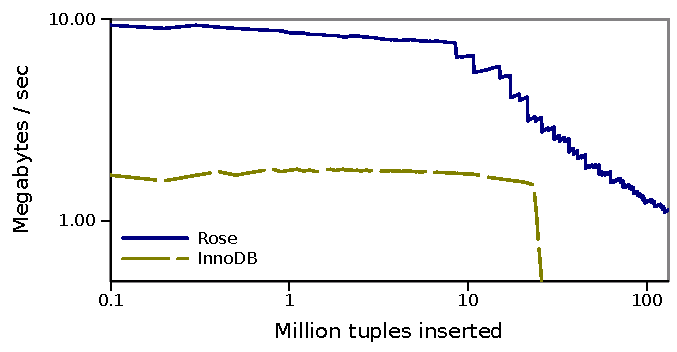
\epsfig{file=average-throughput.pdf, width=3.33in}
\caption{Mean insertion throughput (log-log)}
\label{fig:avg-thru}
\end{figure}
\begin{figure}
\centering
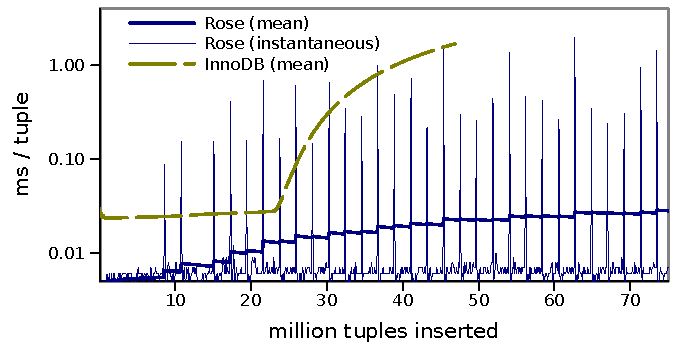
\epsfig{file=average-ms-tup.pdf, width=3.33in}
\caption{Tuple insertion time (``instantaneous'' is mean over 100,000
  tuple windows).}
\label{fig:avg-tup}
\end{figure}

\rows provides roughly 4.7 times more throughput than InnoDB on an
empty tree (Figure~\ref{fig:avg-thru}).  InnoDB's performance remains
constant while its tree fits in memory.  It then falls back on random
I/O, causing a sharp drop in throughput.  \rowss performance begins to
fall off earlier due to merging, and because it has half as much page
cache as InnoDB.  However, \rows does not fall back on random I/O, and
maintains significantly higher throughput than InnoDB throughout the
run.  InnoDB's peak write throughput was 1.8 mb/s and dropped by
orders of magnitude\xxx{final number} before we terminated the
experiment.  \rows was providing 1.13 mb/sec write throughput when it
exhausted the dataset.


%\begin{figure}
%\centering
%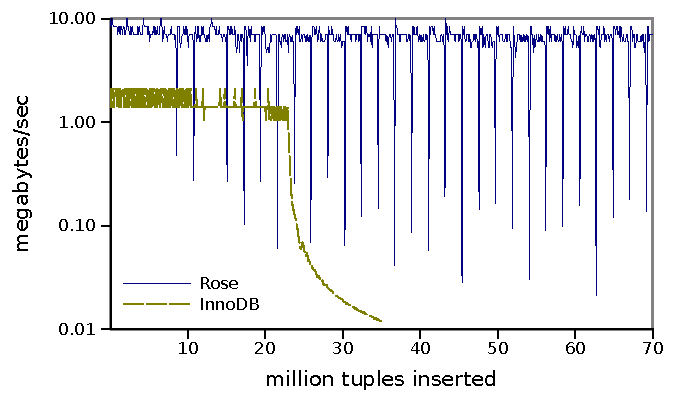
\epsfig{file=instantaneous-throughput.pdf, width=3.33in}
%\caption{Instantaneous insertion throughput (average over 100,000 tuple windows).}
%\label{fig:inst-thru}
%\end{figure}

%\begin{figure}
%\centering
%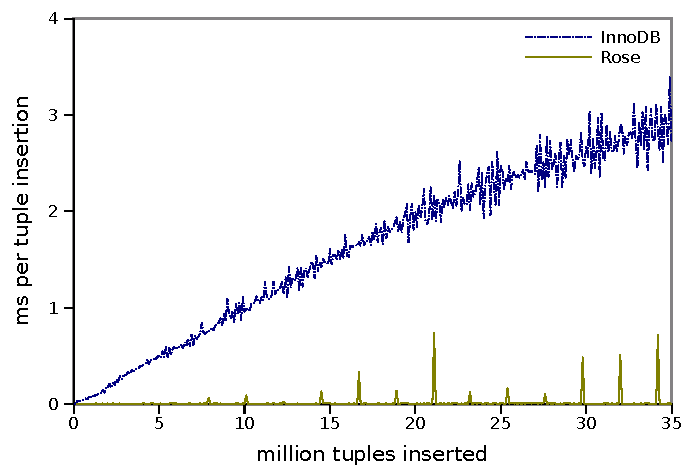
\epsfig{file=instantaneous-ms-tup.pdf, width=3.33in}
%\caption{Instantaneous tuple insertion time (average over 100,000 tuple windows).}
%\end{figure}

\subsection{Comparison with analytical model}

\rows outperforms B-Tree based solutions, as expected.  However, the
prior section says little about the overall quality of our prototype
implementation.  In this section we measure update latency and compare
measured write throughput with the analytical model's predicted
throughput.

Figure~\ref{fig:inst-thru} reports \rowss replication throughput
averaged over windows of 100,000 tuple insertions.  The large downward
spikes occur periodically throughout the run, though the
figure is truncated to only show the first 10 million inserts.  They
occur because \rows does not perform admission control.
%  First, $C0$ accepts insertions at a much
%greater rate than $C1$ or $C2$ can accept them.  Over 100,000 tuples
%fit in memory, so multiple samples are taken before each new $C0$
%component blocks on the disk bound mergers.  Second, \rows merges
%entire trees at once, occasionally blocking smaller components
%for long periods of time while larger components complete a merge
%step.  Both of these problems could be masked by rate limiting the
%updates presented to \rows.

%This paper has mentioned a number of limitations in our prototype
%implementation.

Figure~\ref{fig:4R} compares our prototype's performance to that of an
ideal LSM-tree.  Recall that the cost of an insertion is $4R$ times
the number of bytes written.  We can approximate an optimal value for
$R$ by taking $\sqrt{\frac{|C2|}{|C0|}}$, where tree component size is
measured in number of tuples.  This factors out compression and memory
overheads associated with $C0$.

We use this value to
generate Figure~\ref{fig:4R} by multiplying \rowss replication
throughput by $1 + 4R$.  The additional $1$ is the cost of reading the
inserted tuple from $C1$ during the merge with $C2$.

\rows achieves 2x compression on the real data set.  For comparison,
we ran the experiment with compression disabled, and with
run length encoded synthetic datasets that lead to 4x and 8x compression
ratios.  Initially, all runs exceed optimal throughput as they
populate memory and produce the initial versions of $C1$ and $C2$.
Eventually each run converges to a constant effective disk
utilization roughly proportional to its compression ratio.  This shows
that \rows continues to be I/O bound with higher compression ratios.

The analytical model predicts that, given the hard drive's 57.5~mb/s write
bandwidth, an ideal \rows implementation would perform about twice as
fast as our prototype.  We believe the difference is largely due to
Stasis' buffer manager; on our test hardware it delivers unpredictable
bandwidth between approximately 22 and 47 mb/s.  The remaining
difference in throughput is probably due to \rowss imperfect
overlapping of computation with I/O and coarse-grained control over
component sizes and R.

Despite these limitations, \rows is able to deliver significantly
higher throughput than would be possible with an LSM-tree.  We expect
\rowss throughput to increase with the size of RAM and storage
bandwidth for the foreseeable future.

%Our compressed runs suggest that \rows is
%I/O bound throughout our tests, ruling out compression and other cpu overheads.  We stopped running the
%comparison at 8x because \rows currently requires tuples to be unique;
%to ensure uniqueness we use one column of each tuple to store a unique
%value.  Neither FOR nor RLE compress this value particularly well.
%Since our schema only has ten columns, the maximum achievable
%compression ratio is approximately 10x. 

%% A number of factors contribute to the discrepancy between our model
%% and our prototype's performance.  First, the prototype's
%% whole-tree-at-a-time approach to merging forces us to make extremely
%% coarse and infrequent runtime adjustments to the ratios between tree
%% components.  This prevents \rows from reliably keeping the ratios near
%% the current target value for $R$.  Second, \rows currently
%% synchronously forces tree components to disk.  Given our large buffer
%% pool, a significant fraction of each new tree component is in the
%% buffer pool or operating system cache when the merge thread forces it
%% to disk.  This prevents \rows from overlapping I/O with computation.
%% Finally, our analytical model neglects some minor sources of storage
%% overhead.

%One other factor significantly limits our prototype's performance.


\begin{figure}
\centering
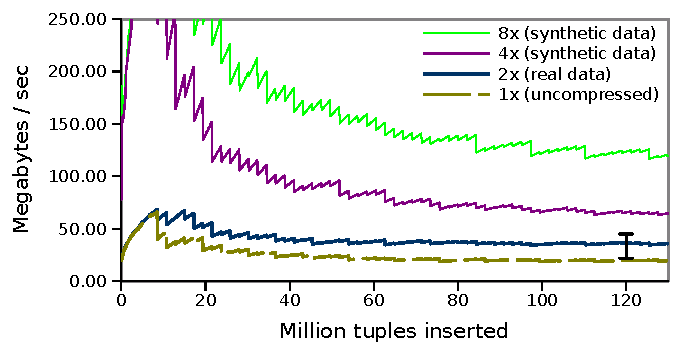
\epsfig{file=4R-throughput.pdf, width=3.33in}
\caption{The hard disk bandwidth an uncompressed LSM-tree would
  require to match \rowss throughput.  Our buffer manager delivered
  22-45 mb/s during the tests.}
\label{fig:4R}
\end{figure}

\subsection{TPC-C / H}

TPC-H is an analytical processing benchmark that targets periodically
bulk-loaded data warehousing systems.  In particular, compared to
TPC-C, it de-emphasizes transaction processing and rollback.  Also, it
allows database vendors to permute the dataset off-line.  In real-time
database replication environments faithful reproduction of
transaction processing schedules is important and there is no
opportunity to resort data before making it available to queries.
Therefore, we insert data in chronological order.

Our \rows prototype is far from a complete storage engine
implementation.  Rather than implement relational algebra operations
and attempt to process and appropriately optimize SQL queries on top
of \rows, we chose a small subset of the TPC-H and C benchmark
queries, and wrote custom code to invoke appropriate \rows tuple
modifications, table scans and index lookup requests.  For simplicity
updates and queries are performed by a single thread.

When modifying TPC-H and C for our experiments, we follow an existing
approach~\cite{entropy,bitsForChronos} and start with a pre-computed
join and projection of the TPC-H dataset.  We use the schema described
in Table~\ref{tab:tpc-schema}.  We populate the table by using a scale
factor of 30 and following the random distributions dictated by the
TPC-H specification.

We generated a dataset containing a list of product orders.  We insert
tuples for each order (one for each part number in the order), then
add a number of extra transactions.  The following updates are applied in chronological order:

\begin{itemize}
\item Following TPC-C's lead, 1\% of orders are immediately cancelled
  and rolled back.  This is handled by inserting a tombstone for the
  order.
\item Remaining orders are delivered in full within the next 14 days.
  The order completion time is chosen uniformly at random between 0
  and 14 days after the order was placed.
\item  The status of each line item is changed to ``delivered'' at a time
  chosen uniformly at random before the order completion time.
\end{itemize}
The following read-only transactions measure the performance of \rowss
access methods:
\begin{itemize}
\item Every 100,000 orders we initiate a table scan over the entire
  data set.  The per-order cost of this scan is proportional to the
  number of orders processed so far.
\item 50\% of orders are checked with order status queries.  These are
  simply index probes.  Orders that are checked with status queries
  are checked 1, 2, or 3 times with equal probability.
\item Order status queries happen with a uniform random delay of 1.3
  times the order processing time.  For example, if an order
  is fully delivered 10 days after it is placed, then order status queries are
  timed uniformly at random within the 13 days after the order is
  placed.
\end{itemize}

The script that we used to generate our dataset is publicly available,
along with Stasis' and the rest of \rowss source code.

This dataset is not easily compressible using the algorithms provided
by \rows.  Many columns fit in a single byte, rendering \rowss version
of FOR useless.  These fields change frequently enough to limit the
effectiveness of run length encoding.  Both of these issues would be
reduced by bit packing.  Also, occasionally revaluating and modifing
compression strategies is known to improve compression of TPC-H data.
TPC-H orders are clustered in the last few weeks of years during the
20th century.\xxx{check}

\begin{table}
\caption{TPC-C/H schema}
\centering
\label{tab:tpc-schema}
\begin{tabular}{|l|c|c|} \hline
Column Name     & Compression Format &  Data type\\ \hline
Part \# + Supplier & RLE       & int32              \\ \hline
Year            & RLE       & int16              \\\hline
Week            & NONE      & int8               \\\hline
Day of week     & NONE      & int8               \\\hline
Order number    & NONE      & int64              \\\hline
Quantity        & NONE      & int8               \\\hline
Delivery Status & RLE       & int8               \\\hline
\end{tabular}
\end{table}

%% We generated a dataset based on this schema then
%% added transaction rollbacks, line item delivery transactions and
%% order status queries.  Every 100,000 orders we initiate a table scan
%% over the entire dataset.  Following TPC-C's lead, 1\% of new orders are immediately cancelled
%% and rolled back; the remainder are delivered in full within the
%% next 14 days.  We choose an order completion time uniformly at
%% random within the next 14 days then choose part delivery times
%% uniformly at random within that range.

%% We decided that $50\%$ of orders would be checked
%% using order status queries; the number of status queries for such
%% transactions was chosen uniformly at random from one to four, inclusive.
%% Order status queries happen with a uniform random delay of up to 1.3 times
%% the order processing time (if an order takes 10 days
%% to arrive then we perform order status queries within the 13 day
%% period after the order was initiated).

Order status queries have excellent temporal locality and generally
succeed after accessing $C0$.  These queries simply increase the
amount of CPU time between tuple insertions and have minimal impact on
replication throughput.  \rows overlaps their processing with the
asynchronous I/O peformed by merges.

We force \rows to become seek bound by running a second set of
experiments a different version of the order status query.  In one set
of experiments (which we call ``Lookup C0''), the order status query
only examines C0.  In the other (which we call ``Lookup all
components''), we force each order status query to examine every tree
component.  This keeps \rows from exploiting the fact that most order
status queries can be serviced from $C0$.

%% The other type of query we process is a table scan that could be used
%% to track the popularity of each part over time.  We know that \rowss
%% replication throughput is significantly lower than its sequential
%% table scan throughput, so we expect to see good scan performance for
%% this query.  However, these sequential scans compete with merge
%% processes for I/O bandwidth, so we expect them to have a measurable impact on
%% replication throughput.

Figure~\ref{fig:tpch} plots the number of orders processed by \rows
per second agasint the total number of orders stored in the \rows
replica.  For this experiment we configure \rows to reserve 1GB for
the page cache and 2GB for $C0$.  We {\tt mlock()} 4.5GB of RAM, leaving
500MB for the kernel, system services, and Linux's page cache.

%% In order to
%% characterize query performance, we re-ran the experiment with various
%% read-only queries disabled.  In the figure, ``All queries'' line contains all
%% the queries mentioned above, while ``None'' only contains updates.
%% The ``Lookup: All components'' line plots the performance of the \rows
%% replica when performing index probes that access each tree component,
%% while ``Lookup: C0'' measures performance when the index probes match
%% data in $C0$.  

As expected, the cost of searching $C0$ is negligible, while randomly
accessing the larger components is quite expensive.  The overhead of
index scans increases as the table increases in size, leading to a
continuous downward slope throughout runs that perform scans.  Index
probes are out of $C0$ until $C1$ and $C2$ are materialized.  Soon
after that, the system becomes seek bound as each index lookup
accesses disk.

Suprisingly, performing periodic table scans improves lookup
performance for $C1$ and $C2$.  The effect is most pronounced after
approximately 3 million orders are processed.  That is approximately
when Stasis' page file exceeds the size of the buffer pool, which is
managed using LRU.  When a merge completes half of the pages it read
become obsolete.  Index scans rapidly replace these pages with live
data using sequential I/O.  This increases the likelihood that index
probes will be serviced from memory.  A more sophisticated page
replacement policy would further improve performance by evicting
obsolete pages before accessible pages.

\begin{figure}
\centering 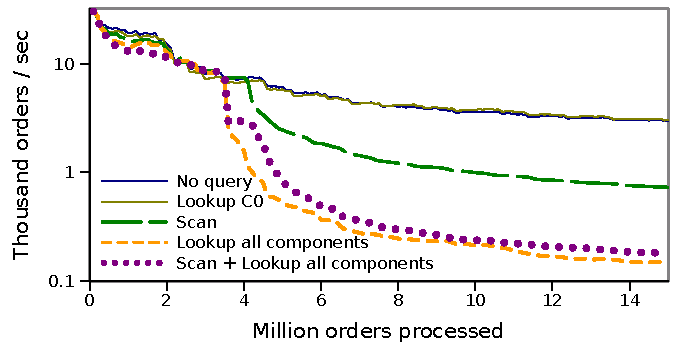
\epsfig{file=query-graph.pdf, width=3.33in}
\caption{\rowss TPC-C/H query costs}
\label{fig:tpch}
\end{figure}


%% Finally, note that the analytical model's predicted throughput
%% increases with \rowss compression ratio.  Sophisticated, high-speed
%% compression routines achieve 4-32x compression ratios on TPC-H data,
%% while \rowss simplistic compression routines provide approximately 2x
%% compression.  Given ample processing power, these algorithms should
%% improve \rowss throughput by four to sixteen times.  XXX check cited ratios

%% Our performance figures show that \rows significantly outperforms a
%% popular, production quality B-Tree implementation.  Our experiments
%% reveal a number of deficiencies in our prototype implementation,
%% suggesting that further implementation efforts would improve its
%% performance significantly.  Finally, though our prototype could be
%% improved, it already performs at roughly $\frac{1}{4}$th of its ideal
%% throughput.  Our analytical models suggest that it will significantly
%% outperform any B-Tree implementation when applied to appropriate
%% update workloads.

\section{Related Work}

\subsection{LSM-Trees}

The original LSM-Tree work\cite{lsm} provides a more detailed
analytical model than the one presented above.  It focuses on update
intensive OLTP (TPC-A) workloads, and hardware provisioning for steady
state workloads.

LHAM is an adaptation of LSM-Trees for hierarchical storage
systems~\cite{lham}.  It was optimized to store higher numbered
components on archival media such as CD-R or tape drives.  It focused
on scaling LSM-trees beyond the capacity of high-performance storage
media and on efficient time-travel queries over archived, historical
data~\cite{lham}.

Partitioned exponential files are similar to LSM-trees, except that
they range partition data into smaller indices~\cite{partexp}.  This solves a number
of problems that are left unaddressed by \rows.  The two most
important issues are skewed update patterns and merge storage
overhead.

\rows is optimized for uniform random insertion patterns
and does not attempt to take advantage of skew in the replication
workload.  If most updates are to a particular partition then
partitioned exponential files merge that partition more frequently,
skipping merges of unmodified partitions.  Partitioning a \rows
replica into multiple LSM-trees would enable similar optimizations.

Partitioned exponential files can use less storage during merges
because the granularity of their merges is smaller.  Performing more,
smaller merges would improve \rowss concurrency and storage overhead.

Partitioned exponential files avoid a few other pitfalls of LSM-tree
implementations.  \rows addresses these problems in different ways.
One issue is page file fragmentation.  Partitioned exponential files
make use of maintenance tasks to move partitions, ensuring that there
is enough contiguous space to hold a new partition.  \rows avoids this
problem by allowing tree components to become fragmented.  It does
this by using Stasis to allocate contiguous regions of pages.  The
regions are long enough to guarantee good sequential scan performance.
\rows always allocates regions of the same length, guaranteeing that
Stasis can reuse all freed regions before extending the page file.
This can waste nearly an entire region per component, which does not
matter in \rows, but could be a significant overhead for a system with
many small partitions.

Some LSM-tree implementations do not support concurrent insertions,
merges, and queries.  This causes such implementations to block during
merges, which take up to $O(n)$ time, where n is the tree size.
\rows never blocks queries, and overlaps insertions and tree merges.
Admission control would provide predictable, optimal insertion
latencies.

Also, some LSM-tree implementations produce many levels of
tree components.  We have argued that two on disk components is
adequate for \rowss target applications.

Later work proposes the reuse of existing B-Tree implementations as
the underlying storage mechanism for LSM-Trees\cite{cidrPartitionedBTree}.  Many
standard B-Tree optimizations (such as prefix compression and bulk insertion)
would benefit LSM-Tree implementations.  \rows uses a custom tree
implementation so that it can take advantage of compression.
Compression algorithms used in B-Tree implementations must provide for
efficient, in-place updates of tree nodes.  The bulk-load application of
\rows updates imposes fewer constraints upon our compression
algorithms.

Recent work optimizes B-Trees for write intensive workloads by dynamically
relocating regions of B-Trees during
writes~\cite{bTreeHighUpdateRates}.  This reduces index fragmentation
but still relies upon random I/O in the worst case.  In contrast,
LSM-Trees never use disk-seeks to service write requests and produce
perfectly laid out B-Trees.

The problem of {\em Online B-Tree merging} is closely related to
LSM-Trees' merge process.  B-Tree merging addresses situations where
the contents of a single table index have been split across two
physical B-Trees that now need to be reconciled.  This situation
arises, for example, during rebalancing of partitions within a cluster
of database machines.

One particularly interesting approach lazily piggybacks merge
operations on top of tree access requests.  To service an index
probe or range scan, the system must read leaf nodes from both B-Trees.
Rather than simply evicting the pages from cache, their approach merges
the portion of the tree that has already been brought into
memory~\cite{onlineMerging}.

The original LSM-Tree paper proposes a mechanism that provides delayed
LSM-Tree index scans with no additional I/O.  When a query requests a table scan, it would wait for
the merge processes to make a pass over the index.
By combining this idea with lazy merging, an LSM-Tree could service
range scans immediately without significantly increasing the amount of
I/O performed by the system.

\subsection{Row-based database compression}

Row-oriented database compression techniques compress each tuple
individually and sometimes ignore similarities between adjacent
tuples.  One such approach compresses low cardinality data by building a
table-wide mapping between short identifier codes and longer string
values. The mapping table is stored in memory for convenient
compression and decompression.  Other approaches include NULL
suppression, which stores runs of NULL values as a single count, and
leading zero suppression which stores integers in a variable length
format that does not store leading zeros.  Row-based schemes typically
allow for easy decompression of individual tuples.  Therefore, they
generally store the offset of each tuple explicitly at the head of
each page.

Another approach is to compress page data using a generic compression
algorithm, such as gzip.  The primary drawback to this approach is
that the size of the compressed page is not known until after
compression.  Also, general purpose compression techniques typically
do not provide random access within pages and are often more processor
intensive than specialized database compression
techniques~\cite{rowImplementationPerf}.

\subsection{Column-oriented database compression}

Column-based compression is based on the observation that sorted
columns of data are often easier to compress than sorted tuples.  Each
column contains a single data type, and sorting decreases the
cardinality and range of data stored on each page.  This increases the
effectiveness of simple, special purpose, compression schemes.

PFOR was introduced as an extension to
the MonetDB\cite{pfor} column-oriented database, along with two other
formats.  PFOR-DELTA is similar to PFOR, but stores differences between values as
deltas.\xxx{check}  PDICT encodes columns as keys and a dictionary that
maps to the original values.  We plan to add both these formats to
\rows in the future.  We chose to implement RLE and PFOR because they
provide high compression and decompression bandwidth.  Like MonetDB,
each \rows table is supported by custom-generated code.

C-Store, another column oriented database, has relational operators
that have been optimized to work directly on compressed
data\cite{compExec}.  For example, when joining two run length encoded
columns, it is unnecessary to explicitly represent each row during the
join.  This optimization would be particularly useful in \rows, as its
merge processes perform repeated joins over compressed data.  Our
prototype does not make use of these optimizations, though they would
likely improve performance for CPU-bound workloads.

A recent paper provides a survey of database compression techniques
and characterizes the interaction between compression algorithms,
processing power and memory bus bandwidth.  The formats within their
classification scheme either split tuples across pages or group
information from the same tuple in the same portion of the
page~\cite{bitsForChronos}.

\rows, which does not split tuples across pages, takes a different
approach, and stores each column separately within a page.  Our
column-oriented page layouts incur different types of per-page overhead, and
have fundamentally different processor
cache behaviors and instruction-level parallelism properties than the
schemes they consider.

In addition to supporting compression, column databases typically
optimize for queries that project away columns during processing.
They do this by precomputing the projection and potentially resorting
and recompressing the data.  This reduces the size of the uncompressed
data, and can improve compression ratios, reducing the amount of I/O
performed by the query.  \rows can support these optimizations by
computing the projection of the data during replication.  This
provides a \rows replica optimized for a particular set of queries,
and is particularly attractive if multiple \rows replicas are
available.

Unlike read-optimized column-oriented databases, \rows is optimized
for write throughput, provides low-latency, in-place updates, and tuple lookups comparable to row-oriented storage.
However, many column storage techniques are applicable to \rows.  Any
column index that supports efficient bulk-loading, provides scans over data in an order appropriate for bulk-loading, and can be emulated by an
updatable data structure can be implemented within
\rows.  This allows us to apply other types index structures
to real-time replication scenarios.

%This property does not come without cost; compared to a column
%store, \rows must merge replicated data more often, achieves lower
%compression ratios, and performs index lookups that are roughly twice
%as expensive as a B-Tree lookup.

\subsection{Snapshot consistency}

\rows relies upon the correctness of the master database's concurrency
control algorithms to provide snapshot consistency to queries.  \rows
is compatible with the two most popular approaches to concurrency
control in OLTP environments: two-phase locking and multiversion concurrency control.

\rows only provides read-only queries.  Therefore, its concurrency
control algorithms need only address read-write conflicts.
Well-understood techniques protect against read-write conflicts
without causing requests to block, deadlock or
livelock~\cite{concurrencyControl}.

%% \subsection{Log shipping}

%% Log shipping mechanisms are largely outside the scope of this paper;
%% any protocol that provides \rows replicas with up-to-date, intact
%% copies of the replication log will do.  Depending on the desired level
%% of durability, a commit protocol could be used to ensure that the
%% \rows replica receives updates before the master commits.
%% \rows is already bound by sequential I/O throughput, and because the
%% replication log might not be appropriate for database recovery, large
%% deployments would probably opt to store recovery logs on machines
%% that are not used for replication.

\section{Conclusion}

Compressed LSM-Trees are practical on modern hardware.  Hardware trends such as increased memory size and sequential disk bandwidth will further improve \rowss performance.  In addition
to developing new compression formats optimized for LSM-Trees, we presented a new approach to
database replication that leverages the strengths of LSM-Trees by
avoiding index probing during updates.  We also introduced the idea of
using snapshot consistency to provide concurrency control for
LSM-Trees.

%% Our prototype's LSM-Tree recovery mechanism is extremely
%% straightforward, and makes use of a simple latching mechanism to
%% maintain our LSM-Trees' consistency.  It can easily be extended to
%% more sophisticated LSM-Tree implementations that perform incremental
%% tree merging.

Our implementation is a first cut at a working version of \rows.
We have characterized the performance of our prototype, and
bounded the replication throughput gain we can expect to achieve via further
optimizations.  By avoiding disk seeks for all operations except
random index probes, uncompressed LSM-Trees can outperform
B-Tree based indices by at least 2 orders of magnitude.  With real-world
database compression ratios ranging from 5-20x, we expect \rows
database replicas to outperform B-Tree based database replicas by an
additional factor of ten.

\xxx{new conclusion?}
% We implemented \rows to address scalability issues faced by large
%scale database installations.  \rows addresses
%applications that perform real-time analytical and decision
%support queries over large, frequently updated data sets.
%Such applications are becoming increasingly common.

\bibliographystyle{abbrv}
\bibliography{rose}  % sigproc.bib is the name of the Bibliography in this case
% You must have a proper ".bib" file
%  and remember to run:
% latex bibtex latex latex
% to resolve all references
%
% ACM needs 'a single self-contained file'!
%
\balancecolumns % GM July 2000
% That's all folks!
\end{document}
